\documentclass[11pt, a4paper]{report}
\usepackage[utf8]{inputenc}

% Change language to Dutch
\usepackage[dutch]{babel}

% Set default font to Open Sans
\usepackage[default]{opensans}

% References
\usepackage{csquotes}
\usepackage[sorting=none]{biblatex}
\addbibresource{bibliography/bibliography.bib}
\defbibheading{bib_heading}{\newpage\addcontentsline{toc}{chapter}{Bibliografie}\begin{flushleft}\Huge{\textbf{\bibname}}\vspace{0.20in}}

% Adjust margins
\usepackage[includeheadfoot,nomarginpar,margin=2.54cm]{geometry}

% Turn references in hyperlinks
\usepackage[hidelinks=true]{hyperref}

% Fancy headers and footers
\usepackage{fancyhdr}
\pagestyle{fancy}
\fancyhead[L,R]{}
\fancyhead[R,L]{}
\fancyfoot[R,L]{}
\fancyfoot[C,C]{\thepage}
\fancypagestyle{plain}{%
  \pagestyle{fancy}%
}
\fancypagestyle{styledchapter}{%
  \fancyhead[L,R]{}
  \fancyhead[R,L]{}
  \fancyfoot[E,L]{}
  \fancyfoot[C,C]{\thepage}
  \renewcommand{\headrulewidth}{0pt}
  \renewcommand{\footrulewidth}{0pt}
}

\renewcommand{\headrulewidth}{.5pt}
\renewcommand{\footrulewidth}{.5pt}

% Define path for images
\usepackage{graphicx}
\graphicspath{ {./images/} }

% Glossary list
\usepackage[toc, acronym, nopostdot, style=index]{glossaries}
\makeglossaries
\newacronym{paas}{PaaS}{Platform as a Service}
\newacronym{api}{API}{application programming interface}
\newacronym{iac}{IaC}{infrastructure as code}
\newacronym{svc}{SVC}{support vector classification}
\newacronym{rest}{REST}{representational state transfer}

\newglossaryentry{machine-learning}
{
    name=machine learning,
    description={is het ontwikkelen van algoritmes en technieken waarmee computers kunnen leren.}
}

\newglossaryentry{machine-learning-pipeline}
{
    name=machine learning pipeline,
    description={is een pijplijn waarin gedefiniëerd staat hoe data stroomt.}
    first={\glsentrydesc{machine learning pipeline} (\glsentrytext{machine learning pipeline})},
    plural={machine learning pipelines},
    descriptionplural={zijn een pijplijnen waarin gedefiniëerd staat hoe data stroomt.}   
}

\newglossaryentry{cloud-computing-platform}
{
    name=cloud computing platform,
    description={}
    first={\glsentrydesc{cloud computing platform} (\glsentrytext{cloud computing platform})},
    plural={cloud computing platformen},
    descriptionplural={},
}

\newglossaryentry{data-mining}
{
    name=datamining,
    description={}
}


\newglossaryentry{vendor-lock-in}
{
    name=vendor lock-in,
    description={is niet de mogelijkheid hebben om naar een andere dienst/provider te gaan die dezelfde service biedt.}
}


\usepackage{wrapfig}

\usepackage{xcolor}

% Display code
\usepackage{listings}

% \definecolor{codegreen}{rgb}{0,0.6,0}
% \definecolor{codegray}{rgb}{0.5,0.5,0.5}
% \definecolor{codepurple}{rgb}{0.58,0,0.82}
% \definecolor{backcolour}{rgb}{0.95,0.95,0.92}

% \lstdefinestyle{mystyle}{
%     backgroundcolor=\color{backcolour},   
%     commentstyle=\color{codegreen},
%     keywordstyle=\color{magenta},
%     numberstyle=\tiny\color{codegray},
%     stringstyle=\color{codepurple},
%     basicstyle=\ttfamily\footnotesize,
%     breakatwhitespace=false,         
%     breaklines=true,                 
%     captionpos=b,                    
%     keepspaces=true,                 
%     numbers=left,                    
%     numbersep=5pt,                  
%     showspaces=false,                
%     showstringspaces=false,
%     showtabs=false,                  
%     tabsize=2
% }

% \lstset{style=mystyle}

% TOC
\usepackage{tocloft}

% Appendix
\usepackage[toc, title]{appendix}

% Use new lines instead of indents in paragraphs
\usepackage[parfill]{parskip}

% Custom components
\usepackage{titlesec}
\usepackage{afterpage}

\newcommand{\styledchapter}
[2]
[Title]
{
  \newpage
  \pagecolor{pink}

  \titleformat{\chapter}{\normalfont\Huge}{\textbf{\thechapter}}{20pt}{\Huge}
  \chapter{\textbf{#1}}\thispagestyle{styledchapter}
  \label{chap:#2}

  \hfill\break

  \afterpage{\nopagecolor}
  \newpage
}
\usepackage{titlesec}
\usepackage{afterpage}

\newcommand{\styledunmarkedchapter}
[2]
[Title]
{
  \newpage
  \AddToShipoutPicture*{\ChapterBackground}
  % \pagecolor{pink}

  \titleformat{\chapter}{\fontfamily{qag}\color{white}\fontsize{37}{37}\selectfont}{}{0pt}{}\thispagestyle{styledchapter}
  \chapter*{\textbf{#1}}\thispagestyle{styledchapter}
  \label{chap:#2}

  \vspace*{\fill}

  {\fontfamily{qag}\fontsize{500}{500}\selectfont\color{garbagepurple}\textbf{\thechapter}}

  \hfill\break

  % \afterpage{\nopagecolor}
  \newpage
}
\newcommand{\appendixsection}
[1]
[Appendix section]
{
  \section*{#1}
  \addcontentsline{toc}{section}{#1}
}

% Highlighting text
\usepackage{soul}

% Package for tables
\usepackage{multirow}

% Qoutes

\usepackage[]{quoting}
% Qoutes inline
\usepackage{dirtytalk}

% Debugging
% \usepackage{showframe}

% Hyphenation fix
% \tolerance=9999
% \emergencystretch=10pt
% \hyphenpenalty=10000
% \hbadness=10

\title{Machine Learning Pipeline Automation}
\author{Amar Kisoensingh}

\begin{document}

% Title page
\maketitle\thispagestyle{empty}\cleardoublepage

\titleformat{\chapter}{\vspace{-1in}}{}{}{\Huge\textbf}
% \chapter*{Voorwoord}\thispagestyle{fancy}\vspace{-.35in}
\section*{Voorwoord}\thispagestyle{fancy}
Voor u ligt de scriptie "Machine Learning Pipeline Automation". Deze scriptie is geschreven in het kader van mijn afstuderen aan de opleiding Informatica aan de Hogeschool Rotterdam en in opdracht van het stagebedrijf NGTI. De afstudeerstage liep van februari 2021 tot juni 2021.

De onderzoeksvraag is bedacht door mijn bedrijfsbegeleider Okke van 't Verlaat. Halverwege de afstudeerstage heeft Kolja van der Vaart de bedrijfsbegeleiding overgenomen. Terugkijkend was de vraag complex en ambitieus. Ik heb me bezig gehouden met machine learning, automatisering en cloud platformen. 

Bij deze wil ik mijn afstudeerbegeleiders Okke van 't Verlaat, Kolja van der Vaart en vanuit school Stelian Paraschiv en Marian Slingerland bedanken voor de zorgvuldige begeleiding. Ik heb met Okke en Kolja effectief kunnen sparren over het onderzoek. Mijn begeleiders hebben mij ook geholpen om de scriptie in de juiste richting te sturen. Tot slot wil ik mijn vrienden bedanken voor het bieden van een ander perspectief om deze scriptie.

Ik wens u veel leesplezier toe.

Amar Kisoensingh

Zoetermeer, \today

\newpage

\section*{Samenvatting}
Een probleem met machine learning (ML) is dat het gebruik ervan tijd en kennis vereist. Ook is er kans op vendor lock-in als ML wordt gebruikt op een cloud platform zoals Google Cloud of Microsoft Azure. Het is dus vrijwel onmogelijk om te verhuizen naar een andere cloud platform.

Het doel van deze scriptie is om niet alleen te onderzoeken in hoeverre het mogelijk is om ML te automatiseren, maar ook of dit kan ongeacht de cloud platform. De onderzoeksvraag kan als volgt opgesteld worden: kan ML geautomatiseerd worden op een cloud platform-agnostisch wijze.

Om deze vraag te beantwoorden is er onderzoek gedaan naar ML pipelines. Hiervoor is literatuuronderzoek en experimentatie van pas gekomen. Met ML pipelines kan op een gestructureerd manier gewerkt worden met ML. Dit verlaagt de leercurve en maakt ML toegankelijker voor nieuwe developers. Naast het onderzoek is ook een proof of concept (PoC) gebouwd om de platform-agnostisch kant te valideren. Met het onderzoek en experimentatie dat gedaan is blijkt dat het mogelijk is om ML te automatiseren op een cloud platform-agnostisch manier.

Het onderzoek kan verder uitgebreid worden door te kijken naar hoe ML toegankelijker gemaakt kan worden voor developers en hoe het systeem robuuster opgezet kan worden.

\newpage

\section*{Summary}
One problem with machine learning (ML) is that using it requires time and knowledge. There is also a chance of vendor lock-in if ML is being used on a cloud platform such as Google Cloud or Microsoft Azure. It is virtually impossible to move to another cloud platform.

The aim of this thesis is not only to investigate to what extent ML can be automated, but also whether this is possible regardless of the cloud platform. The research question can be formulated as follows: can ML be automated in a cloud platform agnostic way.

To answer this question, research has been done on ML pipelines. Literature research and experimentation were utilized. With ML pipelines you can work with ML in a structured way. This not only makes ML more accessible, but lowers the learning curve for new developers. In addition to the research, a proof of concept (PoC) has also been built to validate the platform-agnostic aspect. The research and experimentation that has been done shows that it is possible to automate ML in a cloud platform agnostic way.

The research can be further expanded by looking at how ML can be made more accessible for developers and how the system can be set up more robustly. 

\newpage

% Glossary
\renewcommand{\glossarysection}[2][\theglstoctitle]{
  \def\theglstoctitle{#2}
  \vspace{\cftbeforelottitleskip}
  \par\noindent
  {\cftlottitlefont #2}{\cftafterlottitle}
  \vskip\cftafterlottitleskip\vspace{-0.25in}
}
% \addcontentsline{toc}{chapter}{Afkortingen}
\printglossary[type=\acronymtype,title=Afkortingen,toctitle=Afkortingen]\thispagestyle{fancy}\newpage
% \addcontentsline{toc}{chapter}{Begrippenlijst}
\printglossary[title=Begrippenlijst]\thispagestyle{fancy}\newpage

% List of figures
\renewcommand{\cftbeforeloftitleskip}{-0.15in}
\renewcommand{\cftafterloftitleskip}{0.20in}
% \addcontentsline{toc}{chapter}{Lijst van figuren}
\listoffigures{}\thispagestyle{fancy}\newpage

% List of tables
\renewcommand{\cftbeforelottitleskip}{-0.15in}
\renewcommand{\cftafterlottitleskip}{0.20in}
\listoftables\thispagestyle{fancy}\newpage
% \addcontentsline{toc}{chapter}{Lijst van tabellen}

% Table of Contents
\renewcommand{\cftbeforetoctitleskip}{-0.15in}
\renewcommand{\cftaftertoctitleskip}{0.20in}
\setcounter{tocdepth}{1}
\tableofcontents{}\thispagestyle{fancy}

% Chapters
\styledchapter[Inleiding]{inleiding}

\section{Het bedrijf: NGTI}\label{sec:het-bedrijf-ngti}
NGTI is een mobile app development bureau gevestigd in Rotterdam, Nederland en maakt hoogwaardige mobiele applicaties voor native, hybrid en webgebruik.

\subsection{Klanten van NGTI}\label{subsec:klanten-van-ngti}


\subsection{Tools die worden gebruikt}\label{subsec:tools-die-gebruikt-worden}
Om productief te zijn gebruikt NGTI een aantal tools en programma's om producten te maken en te communiceren met zowel collega's als klanten.

\subsubsection{Slack}\label{subsubsec:slack}
Interne communicatie gaat via Slack. Het programma faciliteren collega's om elkaar met een lage instap te benaderen en berichten die voor het hele bedrijf relevant zijn te versturen. Ook zijn er 'channels' beschikbaar over specifieke onderwerpen, zoals: \textit{\#dev}, \textit{\#ios} en \textit{\#test-automation}.

\subsubsection{Google Workspace}\label{subsubsec:google-workspace}
Met Google Workspace kunnen bestanden en documenten gemaakt, opgeslagen en gedeeld worden. Omdat dit via een browser kan, hoeven werknemers geen software te installeren. NGTI gebruikt het ook om collaboratief en parallel te werken aan hetzelfde document.

\subsubsection{Zoom}\label{subsubsec:zoom}
\hl{Voorheen werdt Zoom alleen gebruikt om te videobellen met collega's en interviewees.} In de tijd van het pandemie is Zoom echter een belangrijke speler geworden om effectief samen te werken. Meetings zoals introducties van nieuwe collega's of demo's van producten worden online gehouden.

\section{Opdracht}\label{sec:opdracht}
NGTI heeft voorzien dat ze haar applicaties 'slimmer' moet maken door \gls{machine-learning} in te zetten. Niet alleen zorgt dit voor een betere gebruikerservaring, maar geeft NGTI ook een voorsprong op haar concurrenten.

Om \gls{machine-learning} toe te passen is het raadzaam om een \gls{machine-learning-pipeline} op te zetten. Een pipeline is een gestructureerde werkwijze om een model te trainen. Het opzetten van de pipeline en een competente model trainen is tijdrovend en vereist kennis in het domein. Vaak worden modellen getrained op een \gls{cloud-computing-platform} zoals Azure, AWS of Google Cloud. Het probleem met platformen zoals deze is dat het ontzettend lastig is om te wisselen van platform en er is veel kennis vereist om een infrastructuur op te zetten.\bigskip\bigskip\bigskip

De opdracht bestaat uit twee onderdelen:
\begin{enumerate}
  \item onderzoek naar het automatiseren van het opzetten van een \gls{machine-learning-pipeline} om het laagdrempelig en minder tijdrovend te maken.
  \item onderzoek naar het maken van een platform agnostische oplossing
\end{enumerate}

Hierbij zal een PoC gemaakt worden om aan te tonen of het haalbaar is. Een diepere duik in het probleem is te vinden in \autoref{chap:probleemanalyse}.

\section{Leeswijzer}\label{sec:leeswijzer}

\styledchapter[Probleemanalyse]{probleemanalyse}

Zoals beschreven in \autoref{sec:aanleiding-opdracht} is NGTI genoodzaakt om machine-learning in te zetten om haar applicaties 'slimmer' te maken. Hier zijn een aantal redenen voor, onder andere:
\begin{enumerate}
  \item gebruikerservaring verbeteren
  \item voorsprong hebben op concurrenten
\end{enumerate}

Het 'slimmer' maken van applicaties kan op verschillende manieren, maar met machine-learning kan een platform gebouwd worden waarmee elke richting op gegaan kan worden. Om machine-learning te implementeren in haar applicaties loopt NGTI tegen een aantal obstakels op, namelijk: expertise vereist in het machine learning domein, tijd om een pipeline op te zetten en vendor lock-in

\section{Expertise Machine Learning}\label{sec:expertise-machine-learning}
Machine learning is geen triviaal onderwerp. Om een model te trainen is kennis nodig van verschillende domeinen: data mining, software engineering en statistieken. In een multidisciplinair team is het voor één teamlid niet nodig om alle domeinen te beheersen.

Doordat er voorkennis nodig is om een model te trainen en een pipeline goed op te zetten, is het vaak te hoogdrempelig voor developers. De expertise is daar daarnaast niet in een korte tijd te vergaren.

\section{Opzetten pipeline}\label{sec:opzetten-pipeline}
Bovenop de complexiteit van machine learning zelf bestaan er verschillende manieren om een model te trainen. Een machine learning pipeline opzetten is daar een van. Een pipeline is een workflow dat bestaat uit een aantal stappen die doorgelopen kan worden om een model te trainen. In elke stap worden acties uitgevoerd, zoals het verwijderen van onbruikbare data of de prestatie van modellen vergelijken en een rapport met uitslagen genereren. Het opzetten van zo een pipeline én de actie(s) in de stappen definiëren kost tijd en vereist specifieke kennis. Daarnaast zijn de stappen en acties vaak hetzelfde voor verschillende pipelines. Het automatiseren en hergebruiken van stappen en acties tussen pipelines zou tot onder andere tijdwinst leiden.

\section{Vendor lock-in}\label{sec:vendor-lock-in}
Er bestaan een aantal diensten, zogenoemde \acrfull{paas}, waarbij je een pipeline kan opzetten en acties kan definiëren. Een van de problemen met een PaaS is vendor lock-in. Dit betekent dat, als er eenmaal een pipeline is opgezet, de overdraagbaarheid van de pipeline naar een andere PaaS vrijwel onmogelijk is. Ook zijn de opties en mogelijkheden om uit te breiden in de toekomst gelimiteerd.

\section{Doelstelling}\label{sec:doelstelling}
Om het probleem op te lossen is onderzoek en experimentatie nodig op verschillende vlakken. De gewenste oplossing is het ontwikkelen van een systeem waarbij developers met weinig tot geen kennis een model kunnen trainen. Het systeem moet de infrastructurele taken voor zich nemen, zoals het opzetten van een pipeline, de stappen en acties automatiseren. Daarnaast moet het systeem ook platform agnostisch zijn zodat het systeem niet aan één platform gebonden is.

\section{Bestaande oplossingen om pipelines op te zetten}\label{sec:bestaande-oplossingen-om-pipelines-op-te-zetten}
Er bestaan een aantal oplossingen die deels aan de eisen in de doelstelling voldoen. Elke oplossing is een PaaS van een derde partij waarbij vendor lock-in inherent is. Dit maakt ze ongeschikt maar betekent echter niet dat ze nutteloos zijn. Er kan namelijk gekeken worden hoe een pipeline wordt opgezet, welke acties de stappen verricht en daar vervolgens (gedeeltelijk) het systeem op baseren. Daarnaast wordt bij alle oplossingen een expertise van ML op een bepaalde niveau verwacht.

De oplossingen kunnen gecategoriseerd worden in twee groepen:
\begin{enumerate}
  \item Machine learning pipeline specifieke services
  \item Cloud computing platform
\end{enumerate}

\subsection{Machine learning pipeline specifieke service}\label{subsec:machine-learning-pipeline-specifieke-service}
Bedrijven zoals Algorithmia \cite{algorithmia-website} en Valohai \cite{valohai-website} bieden alleen diensten om pipelines op te zetten. Ze zorgen voor het databehoud dat door de gebruiker wordt geüpload en het trainen van het model. Verder kan er toezicht gehouden worden op de kosten, beschikbaarheid en prestatie van het model.

Valohai heeft documentatie een aantal blog posts die bij het ontwerpen van het systeem relevant zouden kunnen zijn. 

\subsection{Cloud computing platformen}\label{subsec:cloud-computing-platformen}
De drie grote cloud computing platformen Amazon, Azure en Google hebben meer te bieden dan alleen een pipeline opzetten, zoals het hosten van een website, database of virtuele server. De cloud computing platformen hebben hetzelfde probleem als de machine learning pipeline specifieke services; vendor lock-in is onvermijdelijk. Wat wel een mogelijkheid zou kunnen zijn is dat de andere services van de cloud computing platformen gebruikt kunnen worden als onderdeel van het systeem.

Het systeem zou bijvoorbeeld een server kunnen aanmaken, een model trainen, het resultaat downloaden en vervolgens de server verwijderen. Om dit zonder de grafisch interface te doen kan er gebruik worden gemaakt van frameworks dat interacteert met het platform.

% \subsection{Lokale frameworks}\label{subsec:lokale-frameworks}
% Naast de \glspl{cloud-computing-platform} en machine learning pipeline specifieke services bestaan er ook lokale frameworks om een model te trainen, zoals TensorFlow, Keras en PyTorch \cite{ml-libraries}. 

% \subsection{Algorithmia}\label{subsec:algorithmia}
% \subsection{Valohai}\label{subsec:valohai}
% \subsection{Azure Machine Learning Pipelines (Azure)}\label{subsec:azure-machine-learning-pipelines}
% \subsection{AI Platform Pipelines}\label{subsec:ai-platform-pipelines}
% \subsection{Amazon SageMaker Pipelines}\label{subsec:amazon-sagemaker-pipelines}

\subsection{Frameworks om cloud computing platformen te beheren}\label{subsec:frameworks-om-cloud-computing-platformen-te-beheren}
Gedurende de vooronderzoek zijn frameworks dat cloud computing platformen beheert en frameworks waarmee een pipeline uitgerold kan worden naar boven gekomen. Deze frameworks kunnen deel uitmaken van de oplossing. Een framework dat cloud computing platformen kan beheren is Terraform \cite{terraform}. Met Terraform is het mogelijk om een plan te schrijven waarin bijvoorbeeld staat welke type server nodig is. Bij het uitvoeren van het plan spreekt Terraform een cloud computing platform naar keuze aan om de server op te starten. Terraform kan vervolgens controleren of de server draait en de server afsluiten wanneer het niet meer nodig is.

Kubeflow \cite{kubeflow} is een ander framework waarmee een pipeline kan worden opgezet. Het verschil met Terraform is dat Terraform flexibeler is met wat er aangemaakt kan worden op een cloud computing platform. Kubeflow kan alleen een pipeline uitrollen. Een andere framework zoals Kubeflow is Apache Beam \cite{apache-beam}.

\section{Hoofd- en deelvragen}\label{sec:hoofd-en-deelvragen}
Uitgaand van de drie obstakels kan de hoofdvraag als volgt worden geformuleerd:

\begin{quoting}
  \begin{center}
    \textbf{
      \textit{
        In welke mate kan een machine learning pipeline worden geautomatiseerd onafhankelijk van de onderliggende cloud computing platform?
      }
    }
  \end{center}
\end{quoting}\smallskip

De hoofdvraag kan worden onderbouwd met vier deelvragen. Om te beginnen is het verstandig om te weten welke stappen er in een machine learning pipeline zit:

\begin{quoting}
  \begin{center}
    \textit{
      Uit welke stappen bestaat een machine learning pipeline?
    }
  \end{center}
\end{quoting}\smallskip

Vervolgens kunnen de verschillende cloud computing platformen in kaart worden gebracht:

\begin{quoting}
  \begin{center}
    \textit{
      Wat zijn de verschillen en overeenkomsten tussen cloud computing platformen waarmee een machine learning pipeline kan worden opgezet?
    }
  \end{center}
\end{quoting}\smallskip

Verder kan het handig zijn om meerdere platformen aan te spreken. Dit zou kunnen met een bestaand framework. Hierbij is het, net als de vorige deelvraag, belangrijk om te weten welke frameworks er zijn:

\begin{quoting}
  \begin{center}
    \textit{
      Wat zijn de verschillen en overeenkomsten tussen frameworks waarmee cloud computing platformen beheerd kunnen worden?
    }
  \end{center}
\end{quoting}\smallskip

Ten slotte wordt een PoC gemaakt om te laten zien of het probleem oplosbaar is. Hiervoor is een doordachte voorbereiden onmisbaar:

\begin{quoting}
  \begin{center}
    \textit{
      Hoe ziet de architecturale blauwdruk van een applicatie, waarmee een machine learning pipeline kan worden opgezet, die modulaire acties geautomatiseerd in stappen samenstelt, en die platform-onafhankelijk is, eruit?
    }
  \end{center}
\end{quoting}

% Uitgaand van de drie focuspunten in \autoref{sec:probleemdefinitie} kan de hoofdvraag als volgt worden geformuleerd:\smallskip

% \begin{quoting}
%   \begin{center}
%     \textbf{
%       \textit{
%         In welke mate kan een machine learning pipeline worden geautomatiseerd onafhankelijk van de onderliggende cloud computing platform?
%       }
%     }
%   \end{center}
% \end{quoting}\smallskip

% De hoofdvraag kan worden onderbouwd met vier deelvragen. Om te beginnen is het verstanding om te onderzoeken hoe een \gls{machine-learning} model wordt getraind:\smallskip

% \begin{quoting}
%   \begin{center}
%     \textit{
%       Welke stappen moeten worden ondernomen om een machine learning model te trainen?
%     }
%   \end{center}
% \end{quoting}\smallskip

% Vervolgens kan er op de deelvraag voortborduurt worden om het opzetten van een pipeline in kaart te brengen:\smallskip

% \begin{quoting}
%   \begin{center}
%     \textit{
%       Hoe wordt een machine learning pipeline opgezet?
%     }
%   \end{center}
% \end{quoting}\smallskip

% Verder zijn er verschillende \glspl{cloud-computing-platform} waarmee \gls{machine-learning} modellen getraind kunnen worden. Doordat het systeem platform agnostisch moet zijn is het van belang om verschillende platformen en frameworks te onderzoeken:

% \begin{quoting}
%   \begin{center}
%     \textit{
%       Wat zijn de verschillen en overeenkomsten tussen cloud computing platforms waarmee machine learning modellen kunnen worden getraind?
%     }
%   \end{center}
% \end{quoting}\smallskip

% Ten slotte wordt een PoC gemaakt om te laten zien of het probleem oplosbaar is. Hiervoor is een doordachte voorbereiden onmisbaar:\smallskip

% \begin{quoting}
%   \begin{center}
%     \textit{
%       Hoe ziet de architecturale blauwdruk van een applicatie, waarin een machine learning pipeline kan worden opgezet, die acties voorgeprogrammeerd zijn, en die platform-onafhankelijk is, eruit?
%     }
%   \end{center}
% \end{quoting}

% \newpage
\styledchapter[Onderzoeksmethoden en scope]{methode-van-onderzoek}

{\renewcommand{\arraystretch}{1.35}% for the vertical padding

Om elke hoofd- en deelvraag te beantwoorden, maak ik bij elk gebruik van een onderzoeksmethode. Volgens Scribbr \cite{research-methods} zijn er twee onderzoeksmethoden: kwantitatief en kwalitatief. Bij een kwantitatief onderzoeksmethode wordt data verzameld waarmee grafieken of tabellen gemaakt kunnen worden. De focus bij een kwalitatief onderzoeksmethode ligt bij het verzamelen van verschillende interpertaties en opvattingen. Hierop kan optioneel een eigen interpertatie op gemaakt worden. \cite{quantitative-vs-qualitative}.

Onder kwantitatief en kwalitatief vallen verschillende dataverzamelingsmethoden. Deze beschrijft simpelweg de manier hoe data wordt verzameld. Dit kan bijvoorbeeld met een enquête, literatuuronderzoek op websites en in boeken of een onderzoek over een lange periode \cite{quantitative-vs-qualitative}.

Elke hoofd- en deelvraag is gekoppeld aan een onderzoeksmethoden. Vervolgens is beschreven welk(e) dataverzamelingsmethode(n) wordt gebruikt met een korte toelichting. Daarnaast wordt op een hoog niveau de scope bepaald en de requirements vanuit NGTI mocht die er zijn.

\begin{table}[hbt!]
\centering
\begin{tabular}{|p{.215\linewidth}|p{.72\linewidth}|}
\hline
\multicolumn{2}{|p{.97\linewidth}|}{\textbf{D1: Uit welke stappen bestaat een machine learning pipeline?}} \\ \hline
  \textbf{Methode(s)}&
    Kwalitatief
  \\ \hline
  \textbf{Dataverzamelings methode(n)}&
    Literatuuronderzoek, fundamenteel onderzoek, toegepast onderzoek
  \\ \hline
  \textbf{Scope}&
    Binnen de scope:
    \begin{itemize}
      \item In kaart brengen uit welke stappen een pipeline bestaat
      \item Acties die in een stap worden uitgevoerd
      \item Of het mogelijk is om stappen te versimpelen / abstraheren voor developers
      \item Of het mogelijk is om stappen en acties te automatiseren
    \end{itemize}
    Buiten de scope:
    \begin{itemize}
      \item Automatisering van stappen en acties
      \item Een versimpeling van machine learning
    \end{itemize}
  \\ \hline
  \textbf{Toelichting}&
    Er wordt gekeken naar welke stappen er in een pipeline zitten. De theorie wordt vervolgens toegepast in een experiment. De nadruk ligt vooral of de mogelijkheid er is om stappen en acties te automatiseren en of machine learning versimpeld kan worden, niet dat er een uitwerking is.
  \\ \hline
\end{tabular}
\caption{Deelvraag 1}
\label{table:sq1}
\end{table}

\space
\newpage

\begin{table}[hbt!]
\centering
\begin{tabular}{|p{.215\linewidth}|p{.72\linewidth}|}
\hline
\multicolumn{2}{|p{.97\linewidth}|}{\textbf{D2: Wat zijn de verschillen en overeenkomsten tussen cloud computing platformen waarmee een machine learning pipeline kan worden opgezet?}} \\ \hline
  \textbf{Methode}&
    Kwalitatief
  \\ \hline
  \textbf{Dataverzamelings methode(n)}&
    Literatuuronderzoek, vergelijkend onderzoek
  \\ \hline
  \textbf{Scope}&
    Binnen de scope:
    \begin{itemize}
      \item Inventarisatie met de "long list short list"\space methode
      \item Welke functionaliteit bieden de platformen op een machine learning pipeline op te zetten
      \item Ervaring opdoen doormiddel van een pipeline te maken binnen twee cloud computing platformen
      \item Basale inventarisatie en vergelijking van alternatieve manieren om met een cloud computing platform te communiceren
    \end{itemize}
    Buiten de scope:
    \begin{itemize}
      \item Prijs, performance en snelheid
    \end{itemize}
  \\ \hline
  \textbf{Toelichting}&
    Cloud computing platformen worden in kaart gebracht. Vervolgens wordt met criteria bepaald in een later stadium de lijst verkort tot twee kandidaten. Alternatieve manieren om met een cloud computing platform te communiceren is afgebakend tot first-party tools en frameworks dat een of meerdere platformen tegelijk kan aanspreken.
  \\ \hline
\end{tabular}
\caption{Deelvraag 2}
\label{table:sq2}
\end{table}

\begin{table}[hbt!]
\centering
\begin{tabular}{|p{.215\linewidth}|p{.72\linewidth}|}
\hline
\multicolumn{2}{|p{.97\linewidth}|}{\textbf{D3: Wat zijn de verschillen en overeenkomsten tussen frameworks waarmee cloud computing platformen beheerd kunnen worden?}} \\ \hline
  \textbf{Methode}&
    Kwalitatief
  \\ \hline
  \textbf{Dataverzamelings methode(n)}&
    Literatuuronderzoek, vergelijkend onderzoek
  \\ \hline
  \textbf{Scope}&
    Binnen de scope:
    \begin{itemize}
      \item Inventarisatie naar wat er aangemaakt, gewijzigd en verwijderd kan worden binnen een cloud computing platform
      \item Hoe een machine learning pipeline op papier gemaakt zou worden met een framework
      \item Experiment met het opzetten van een pipeline via het framework op een cloud computing platform
    \end{itemize}
  \\ \hline
  \textbf{Toelichting}&
  Er wordt gekeken naar welke frameworks er beschikbaar zijn en wat de verschillen/overeenkomsten zijn. Om de applicatie future proof te maken is het belangrijk om een framework te kiezen wat in de praktijk beproefd is en ondersteuning van een community heeft.
  \\ \hline
\end{tabular}
\caption{Deelvraag 3}
\label{table:sq3}
\end{table}

\space
\newpage

\begin{table}[hbt!]
\centering
\begin{tabular}{|p{.215\linewidth}|p{.72\linewidth}|}
\hline
\multicolumn{2}{|p{.97\linewidth}|}{\textbf{D4: Hoe ziet de architecturale blauwdruk van een applicatie, waarin een machine learning pipeline kan worden opgezet, die acties voorgeprogrammeerd zijn, en die platform-onafhankelijk is, eruit?}} \\ \hline
  \textbf{Methode}&
    Kwalitatief
  \\ \hline
  \textbf{Dataverzamelings methode(n)}&
    Literatuuronderzoek
  \\ \hline
  \textbf{Scope}&
    Binnen de scope:
    \begin{itemize}
      \item Technische tekeningen
    \end{itemize}
    Buiten de scope:
    -
  \\ \hline
  \textbf{Toelichting}&
    De literatuuronderzoek slaat op of de technische tekeningen gemaakt zijn volgens een standaard zoals UML. Dit komt niet terug als theorie maar de bronnen worden wel vermeld.
  \\ \hline
\end{tabular}
\caption{Deelvraag 4}
\label{table:sq4}
\end{table}

\space
\newpage

\begin{table}[hbt!]
\centering
\begin{tabular}{|p{.215\linewidth}|p{.72\linewidth}|}
\hline
\multicolumn{2}{|p{.97\linewidth}|}{\textbf{H: In welke mate kan een machine learning pipeline worden geautomatiseerd onafhankelijk van de onderliggende cloud computing platform?}} \\ \hline
  \textbf{Methode}&
    Kwalitatief
  \\ \hline
  \textbf{Dataverzamelings methode(n)}&
    Literatuuronderzoek
  \\ \hline
  \textbf{Scope}&
    De scope wordt bepaald na de requirement analyse.
  \\ \hline
  \textbf{Toelichting}&
    Onderzoek naar documentatie van gebruikte framework(s).
  \\ \hline
\end{tabular}
\caption{Hoofdvraag}
\label{table:mq}
\end{table}
\styledchapter[Stappen in een machine learning pipeline]{stappen-in-een-machine-learning-pipeline}

Een ML pipeline is zoals beknopt beschreven in \autoref{subsec:opzetten-pipeline} een collectie van stappen dat wordt doorlopen om een model te trainen. Elke stap bevat een aantal acties dat wordt uitgevoerd, zoals onbruikbare data weghalen of de prestatie analyseren. De stappen en acties worden in \autoref{sec:de-stappen-in-een-machine-learning-pipeline} uitgelegd. Een van de stappen in een pipeline is het trainen van het model. Om een idee te krijgen van ML en modellen trainen wordt dit kort uitgelegd.

\section{Wat is machine learning?}\label{sec:wat-is-machine-learning}
ML houdt in dat een computer een taak kan uitvoeren zonder ervoor expliciet geprogrammeerd te zijn. Dit wordt gedaan door een ML model te laten leren van een gegeven dataset. Vervolgens kan er een voorspelling worden gemaakt \cite[p.~1-3]{introduction-to-machine-learning}.

De domeinen deep learning (DL), neural networks (NN) en artificial intelligence (AI) komen vaak voor als het over ML gaat. Zoals weergegeven in \autoref{fig:ai-ml-nn-dl} is te zien dat ML een subset is van AI, NN een subset van ML en als laatste DL dat een subset is van NN.

Bij AI wordt niet alleen ML toegepast, maar ook concepten zoals beredeneren, plannen, vooruitdenken, onthouden en terug refereren. Een voorbeeld hiervan is dat een ML model kan voorspellen wat het volgende woord in een zin kan zijn, maar een AI kan beredeneren waarom de zin gebouwd is zoals het is en hoe het binnen de context van de alinea past \cite{ml-think-about-ml-brownlee}.

\begin{figure}[hbt!]
  \centering
  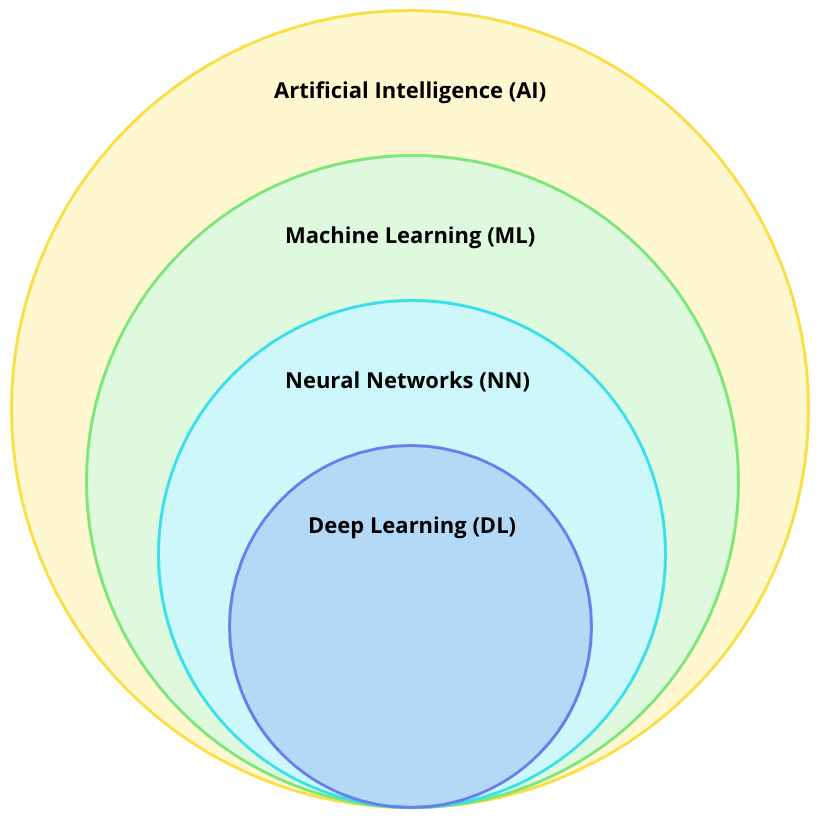
\includegraphics[width=0.48\textwidth]{chapter-4/AI-ML-NN-DL.png}
  \caption{Machine learning in de context van andere domeinen}
  \label{fig:ai-ml-nn-dl}
\end{figure}

Een NN bestaat uit een collectie van nodes dat gemodelleerd is naar de hersenen. Een NN heeft minimaal 3 lagen: een input laag, een verborgen laag en een output laag. Elke laag bevat neuronen dat data als input kan krijgen en data als output aan de volgende laag meegeeft. DL is een NN dat meerdere verborgen lagen bevat \cite{ml-neural-network-nicholson}.

In het ML domein bestaan talloze algoritmes om voorspellingen te maken. In de [BIJLAGE LINK] is een mind-map te vinden van de algoritmes die gedurende de scriptie naar voren zijn gekomen. Het grotendeels kan gegroepeerd worden in vier stijlen: supervised, unsupervised, semi-supervised en reinforcement learning. In de [BIJLAGE LINK] is meer informatie over de stijlen te vinden.

Het trainen van een model is een proces waarbij vooraf data wordt opgeschoond en achteraf de prestatie van het model wordt gevalideerd. Normaliter wordt dit gedaan door specifieke code te schrijven voor deze taken. Een valkuil is dat de code niet bij elke developer werkt en schaalt niet in alle gevallen naar een productie omgeving. Een manier om dit wel te behalen is om te werken met ML pipelines. Zoals kort uitgelegd in \autoref{subsec:opzetten-pipeline} bestaat een ML pipeline uit stappen en acties. Er is echter geen consensus binnen het ML domein over wat de juiste stappen en acties in een pipeline zijn. Voor de scriptie is gekozen voor een pipeline van Hapke en Nelson uit het boek "Building Machine Learning Pipelines". Het boek is gemaakt en gepubliceerd door O'Reilly; een bekend en gecrediteerd bedrijf dat boeken maakt binnen het software engineering domein.

\section{De stappen in een machine learning pipeline}\label{sec:de-stappen-in-een-machine-learning-pipeline}
Een ML pipeline begint met het opnemen van data en eindigt met het ontvangen van feedback om de prestatie van het model te verbeteren. De pipeline bevat een aantal stappen zoals data voorbereiden, het model trainen en het uitrollen van het model (\autoref{fig:model-lifecycle-oreilly}).

\begin{figure}[hbt!]
  \centering
  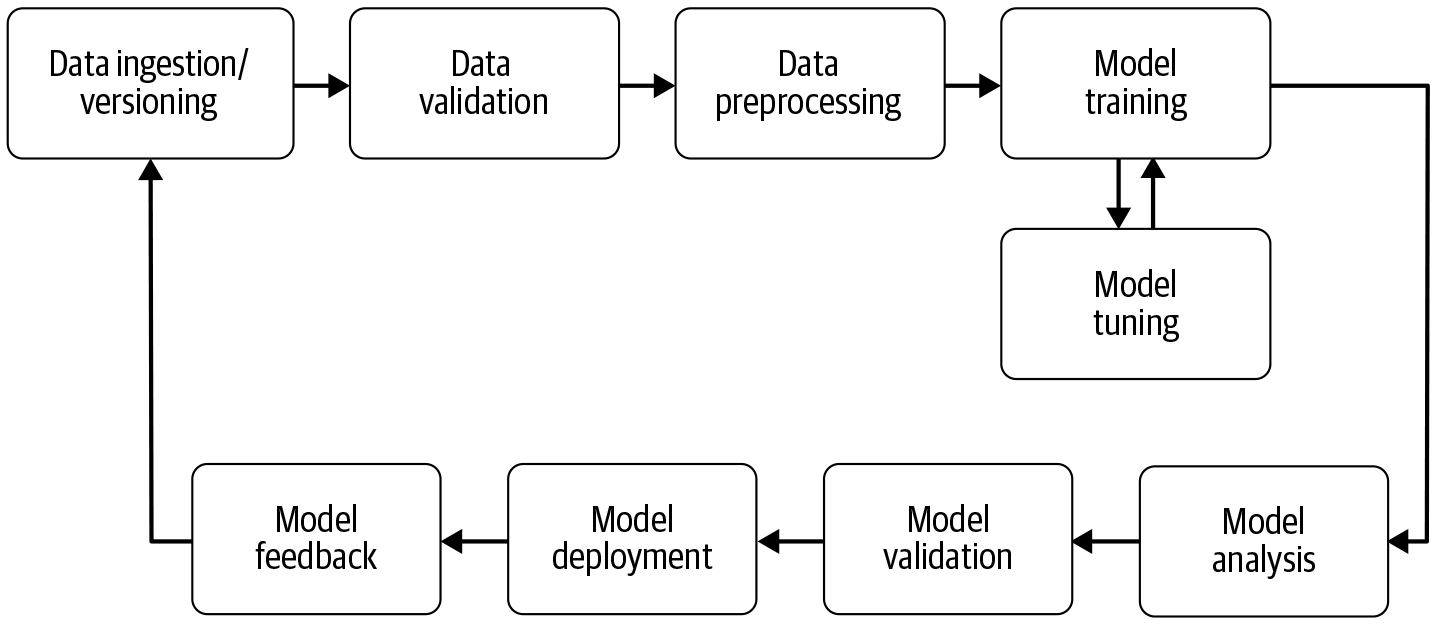
\includegraphics[width=.8\textwidth]{chapter-4/ml-pipeline-lifecycle-oreilly.png}
  \caption{Lifecycle van een model volgens Hapke en Nelson \cite[p.~4]{building-machine-learning-pipelines-oreilly}.}
  \label{fig:model-lifecycle-oreilly}
\end{figure}

In totaal zijn er, zonder de feedback loop stap, acht stappen dat elke keer doorlopen moeten worden om een model te trainen. In de volgende subkoppen zullen de stappen worden doorlopen met een korte uitleg over wat er gebeurd in een stap. 

\subsection{Stap 1: Data opname en versiebeheer (Data ingestion/versioning)}\label{subsec:data-opname-en-versiebeheer}
De eerste stap in de pipeline is het opnemen van data. Met deze data zal het model getraind, gevalideerd en getest worden. De dataset kan van een of meerdere bronnen komen, zoals lokaal, een online opslag locatie of van een database. Zodra de data is ingeladen, moet het verdeeld worden tussen een train, validatie en test dataset. Normaal gebeurt dit met een split ratio van 6:2:2. De train dataset is 60\% en de validatie en test datasets zijn allebei 20\% van de originele dataset \cite[p.~27-37]{building-machine-learning-pipelines-oreilly}.

Een use case van een pipeline is dat een nieuw model getraind kan worden door een geüpdatet dataset te gebruiken. Dit wordt gedaan door de voorgaande dataset te gebruiken waarbij nieuwe data is toegevoegd. Door het gebruik van verschillende datasets is het verstandig om versiebeheer toe te passen. Zo is goed te zien welk dataset welk model produceert. Een versie geven aan een dataset gebeurt voordat de dataset wordt ingeladen \cite[p.~39-40]{building-machine-learning-pipelines-oreilly}. Versiebeheer voor datasets kan bijvoorbeeld met DVC \cite{dvc} of Pachyderm \cite{pachyderm}.

% De iris dataset wordt in \autoref{fig:step-1} geïmporteerd door middel van code. Normaal gesproken zou, voordat deze code uitgevoerd wordt, een versie gegeven worden aan de dataset. Omdat de schaal van dit voorbeeld klein is en om de voorbeeld reproduceerbaar te houden is dit niet gedaan. De dataset wordt aangemaakt met de namen voor de kolommen op regel 5 net zoals het voorbeeld in \autoref{table:example-iris-dataset}. Vervolgens is de dataset onder de variabel naam \(dataset\) beschikbaar voor de komende stappen.

% \begin{figure}[hbt!]
%   \centering
%   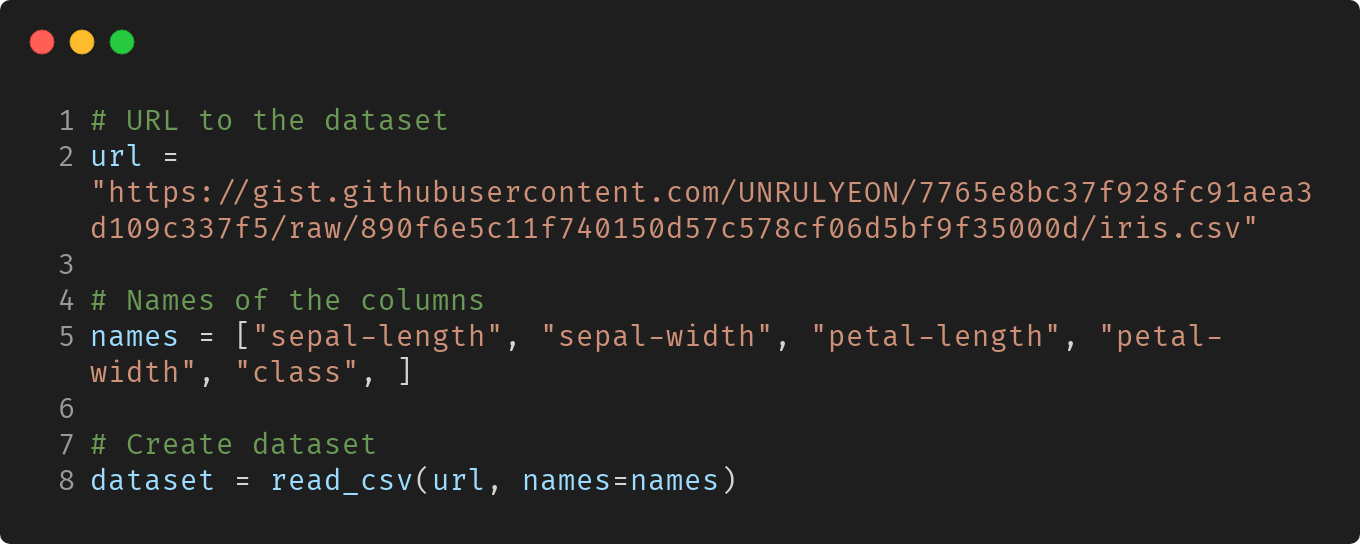
\includegraphics[width=.8\textwidth]{chapter-4/step-1.png}
%   \caption{Dataset importeren}
%   \label{fig:step-1}
% \end{figure}

\subsection{Stap 2: Data validatie (Data validation)}\label{subsec:data-validatie}
Nu de dataset verdeeld is, een versie heeft en op een bereikbare plek is, kan de data gevalideerd worden. Deze stap is vooral belangrijk om te voorkomen dat een model wordt getraind dat niet nuttig is aangezien het trainen veel tijd in beslag kan nemen. Een bekende uitdrukking is "garbage in = garbage out". Dit betekent dat als de dataset niet goed is, het model ook niet goed zal presteren \cite[p.~43]{building-machine-learning-pipelines-oreilly}. Tijdens de validatie stap wordt gecontroleerd op het volgende:

\begin{itemize}
  \item Afwijkingen in de dataset
  \item Wijzigingen in de structuur
  \item Algemene statistieken in vergelijkingen met voorgaand datasets \cite[p.~44]{building-machine-learning-pipelines-oreilly}
\end{itemize}

Bij het controleren van afwijkingen in de dataset wordt gekeken naar waardes die opmerkelijk zijn. Afwijkende waardes liggen te ver van het gemiddelde en kan een verkeerd beeld schetsen bij het trainen van het model. Deze uitschieters kunnen simpelweg uit de dataset gefilterd worden.

Het kan voorkomen dat bij een nieuw dataset de type van waardes zijn gewijzigd. Een \(int\) kan bijvoorbeeld veranderd zijn in een \(string\) of \(boolean\). Er is dan sprake van een wijziging in de structuur van de dataset. Dit is problematisch omdat er een vertaalstap gemaakt moet worden naar iets bruikbaars. Als dit niet mogelijk is moeten de waardes uitgefilterd worden wat de prestatie van het model negatief kan beïnvloeden.

De algemene statistieken is een hulpmiddel om te controleren op afwijkingen en wijzigingen. Vaak kan de controle in een oogopslag gedaan worden. 

% De code voor het genereren van de statistieken hangt af van hoe de dataset eruit ziet en wat er gegenereerd moet worden. In \autoref{fig:step-2} is te zien hoe statistieken worden gegenereerd uit de iris dataset.

% \begin{figure}[hbt!]
%   \centering
%   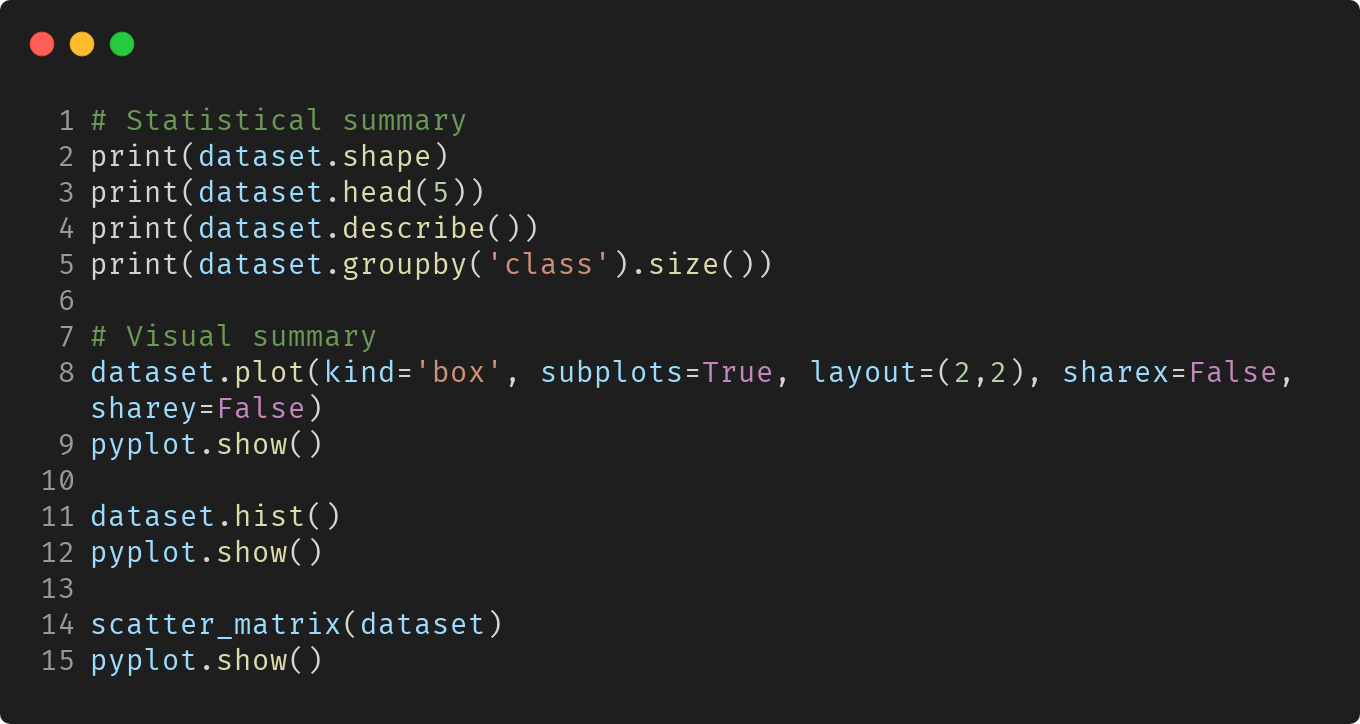
\includegraphics[width=.8\textwidth]{chapter-4/step-2.png}
%   \caption{Statistieken genereren}
%   \label{fig:step-2}
% \end{figure}

% \begin{figure}[hbt!]
%   \centering
%   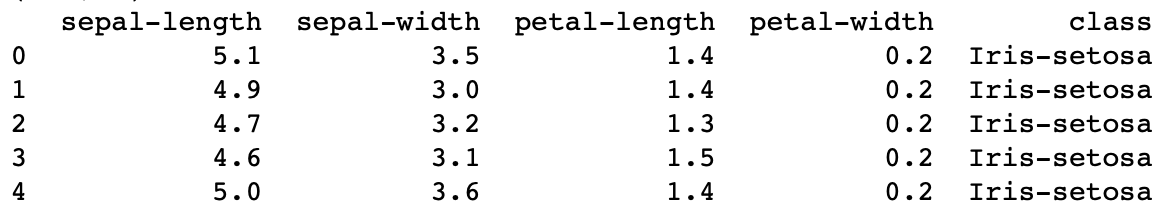
\includegraphics[width=.9\textwidth]{chapter-4/step-2-head-dataset.png}
%   \caption{Statistieken - Eerste 5 regels van de iris dataset}
%   \label{fig:step-2-head-dataset}
% \end{figure}

% \begin{figure}[hbt!]
%   \centering
%   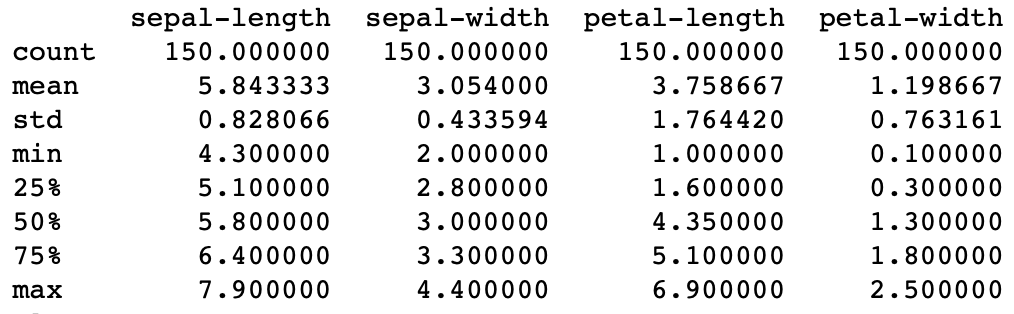
\includegraphics[width=.8\textwidth]{chapter-4/step-2-dataset-described.png}
%   \caption{Statistieken - De iris dataset beschreven}
%   \label{fig:step-2-dataset-described}
% \end{figure}

% \begin{figure}[hbt!]
%   \centering
%   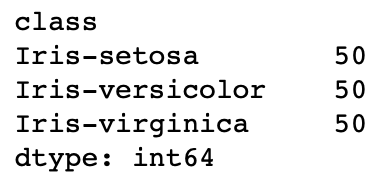
\includegraphics[width=.4\textwidth]{chapter-4/step-2-grouped-by-class.png}
%   \caption{Statistieken - Iris dataset gegroepeerd}
%   \label{fig:step-2-grouped-by-class}
% \end{figure}

\subsection{Stap 3: Data voorbereiden (Data preprocessing)}\label{subsec:data-voorbereiden}
Het voorbereiden van de dataset is een stap dat de prestatie van het model verbetert en het proces van het trainen versneld. Deze stap kan verdeeld worden in twee sub-stappen: het opschonen en het optimaliseren van de dataset.

Bij het opschonen worden bijvoorbeeld duplicaten of waardes die onbruikbaar zijn uit de dataset weggehaald. Onbruikbare waardes zijn waardes die simpelweg niet kloppen of verkeerd zijn ingevoerd. Hierbij kan bijvoorbeeld gedacht worden aan een medewerken die de interactietijd met een klant moet bijhouden, maar is vergeten om de eindtijd te noteren. Voor het algoritme zal het dan lijken alsof de medewerker een klant tot sluitingstijd heeft geholpen.

Datasets kunnen geoptimaliseerd worden om twee redenen: algoritmes werken sneller met waardes die dichter bij \(0\) liggen en algoritmes kunnen niet met elke waarde in de dataset omgaan. Om de efficiëntie van het algoritme te verbeteren kunnen een aantal technieken gebruikt worden:

\begin{itemize}
  \item Schalen
  \item[] Bij het schalen van data worden de waardes getransformeerd waardes dat ligt tussen een schaal, zoals tussen \(0\) en \(100\) of \(0\) en \(1\). Bij het schalen wordt het \textbf{bereik} getransformeerd \cite{scale-and-normalize-data}. 
  \item Normaliseren
  \item[] Als een dataset wordt gestandaardiseerd, worden de waarden getransformeerd in een standaard normale verdeling waarbij het gemiddelde \(0\) en de afwijking \(1\) is. Hierbij wordt de \textbf{vorm} van de dataset getransformeerd \cite{scale-and-normalize-data}. Het normaliseren is belangrijk als het algoritme waardes vergelijkt met verschillende eenheden \cite{feature-scaling-standardization}. In sommige gevallen is normalisering een vereiste bij een aantal algoritmes \cite{data-transformation-standardization-vs-normalization}.
  \item Categorisch codering
  \item[] Een groot aantal algoritmes kan alleen omgaan met numerieke waardes. Het kan voorkomen data datasets categorische waardes bevatten. Dit zijn waardes dat een label voorstellen, zoals \(first\), \(second\) of \(third\). Om deze waardes te gebruiken moeten ze worden gecodeerd als een numerieke waarde. De label kan als de waarde \(1\) of \(2\) gecodeerd worden. Deze techniek heet integer encoding en kan gebruikt worden als de volgorde van de codering klopt. Een andere techniek om waardes te coderen heet hot encoding. Deze techniek wordt gebruikt waarbij de labels geen relatie met elkaar hebben en maakt gebruik van meerdere waardes om een label te beschrijven:
  \begin{center}
    $$\begin{bmatrix}
      \textbf{Animal} & \textbf{C1} & \textbf{C2} & \textbf{C3}\\
      cat & 1 & 0 & 0 \\
      dog & 0 & 1 & 0 \\
      mouse & 0 & 0 & 1 \\
    \end{bmatrix}$$
  \end{center}


\end{itemize}

Dit is een goed moment om het getransformeerde dataset op te slaan als "tussen-dataset"\space zodat deze stap niet herhaalt hoeft te worden. Het voorbereiden van grote datasets kan een grote hoeveelheid tijd in beslag nemen.

\subsection{Stap 4 en 5: Model trainen en tunen (Model training and Model tuning)}\label{subsec:model-trainen-en-tunen}
Na het valideren en voorbereiden van de dataset kan het model getraind worden. Het trainen gaat door middel van een ML algoritme. Een algoritme is vergelijkbaar met een conventionele algoritme in software engineering zoals bijvoorbeeld binary search, merge sort en depth first search. Het algoritme slaat na het trainen met de dataset regels, nummers en algoritme specifieke data structuren op in de vorm van een model. Het algoritme kan worden gezien als een specifiek programma waarmee, gegeven een input, voorspellingen mee gedaan kan worden \cite{ml-algorithm-model-difference}.

Elk algoritme heeft variabelen om er voor te zorgen dat het algoritme beter aansluit op de dataset. Deze variabelen heten \textit{hyperparameters}. Het algoritme heeft standaard hyperparameters die niet altijd de optimale prestatie behalen. Op een heuristische wijze kunnen de optimale hyperparameters gevonden worden \cite{ml-model-hyper-parameter-brownlee}. Dit proces heet \textit{tunen}.

In \autoref{fig:hyperparameter-example-0.1} en \autoref{fig:hyperparameter-example-100} is te zien hoe de \(gamma\) hyperparameter van een SVC algoritme invloed heeft op het model. Dit algoritme classificeert op basis van gegeven waardes. De waardes worden geplot en zal binnen een van de drie kleuren vallen. Het model met als hyperparameter waarde \(100\) zal vaker de classificatie met de bruine kleur als voorspelling geven dan als de waarde \(0.1\) zou zijn.

\begin{figure}[hbt!]
  \centering
  \begin{minipage}{0.45\textwidth}
      \centering
      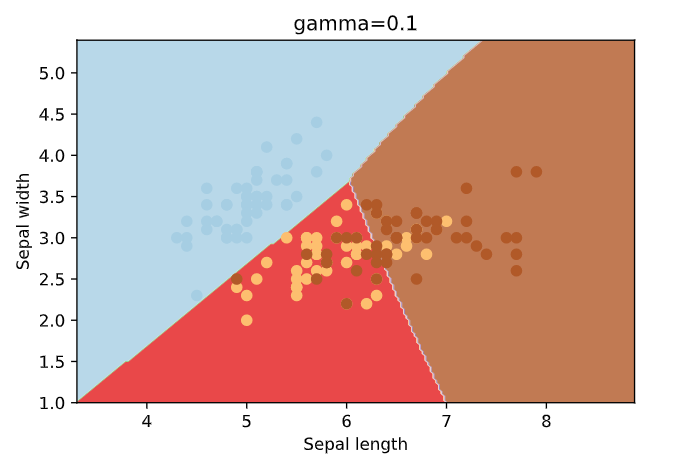
\includegraphics[width=1\textwidth]{./chapter-4/hyperparameter-0.1.png}
      \caption{Gamma hyperparameter van een SVC algoritme met waarde 0.1}
      \label{fig:hyperparameter-example-0.1}
  \end{minipage}\hfill
  \begin{minipage}{0.45\textwidth}
      \centering
      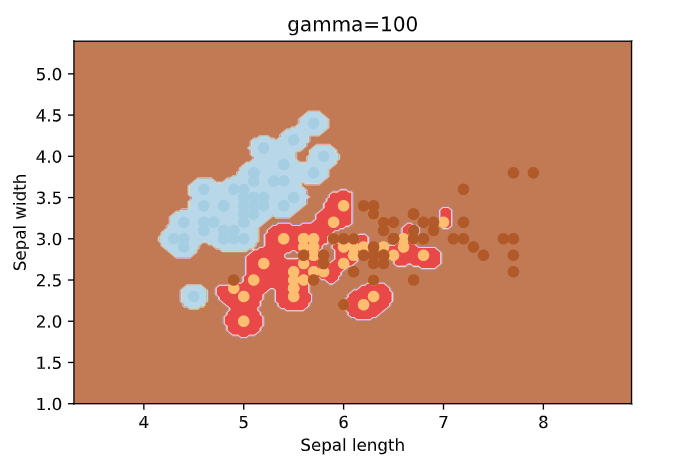
\includegraphics[width=1\textwidth]{./chapter-4/hyperparameter-100.png}
      \caption{Gamma hyperparameter van een SVG algoritme met waarde 100}
      \label{fig:hyperparameter-example-100}
  \end{minipage}
\end{figure}

\subsection{Stap 6 en 7: Model analyse en validatie (Model analysis and Model validation)}\label{subsec:model-analyse-en-validatie}
Na het trainen en tunen kan analyse en validatie plaats vinden. Bij het analyseren wordt de prestatie van het model vergeleken met voorgaande modellen. Om dit te doen kan, net als in \autoref{subsec:data-validatie}, statistieken gegenereerd worden van het model. De soort statistiek hangt af van wat voor soort algoritme is gebruikt. Een classificatie algoritme heeft bijvoorbeeld andere statistieken dan een regressie algoritme. Op basis van de uitkomst kan de dataset of hyperparameters aangepast worden om de accuraatheid te verhogen.

Met de validatie van een model moet er gekeken worden met een genuanceerd perspectief. Validatie gaat namelijk over hoe eerlijk een model is als er gekeken wordt naar een bepaalde groep. Een groep kan gedefinieerd worden als geslacht, etniciteit, locatie of leeftijd. Het kan namelijk voorkomen dat de dataset voornamelijk bestaat uit bijvoorbeeld vrouwen. Dit \textit{kan} ervoor zorgen dat het model minder accurate voorspellingen maakt voor mannen \cite[p.~109-110]{introduction-to-machine-learning}. Een voorbeeld waar het gebruik van ML grote negatieve gevolgen had was de toeslagenaffaire in 2020. De Nederlandse overheid maakte gebruik van een systeem dat aangaf of een burger mogelijk bijstandsfraude had gepleegd. Het systeem maakte gebruikt van ML om fraude aan te geven. Jaren na het gebruik bleek dat er sprake was van etnische profilering. De dataset bestond voornamelijk uit immigranten uit Islamitische landen. Het systeem heeft hierdoor een \textit{bias} \cite{ml-fairness-dutch-syri}.

\subsection{Stap 8: Model uitrollen (Model deployment)}\label{subsec:model-uitrollen}
Na het analyseren en valideren kan het model uitgerold worden. Het uitrollen kan op twee manieren: inbakken in een app of serveren met een \acrfull{api}.

Met het inbakken in een app wordt bedoelt dat het model meegenomen wordt als de app gebouwd wordt. Voordelen van deze methode is dat het model offline bruikbaar is en de rekenkracht van het apparaat gebruikt kan worden om te voorspellen of classificeren. Een nadeel is dat het model niet makkelijk geüpdatet kan worden.

Een model serveren door middel van een \Acrshort{api}. De app dat het model wilt gebruiken zal een request moeten doen met input. De \Acrshort{api} geeft de input door aan het model. Het model geeft een predictie terug dat de \Acrshort{api} doorstuurt naar de applicatie. Het updaten van het model gaat gemakkelijker dan het model inbakken met een app. Een nadeel is de eis dat de app een internetverbinding moet hebben om het model te gebruiken \cite[p.~130]{introduction-to-machine-learning}.

In \autoref{fig:step-8-deploy-model} is te zien hoe een model geserveerd wordt via een \Acrshort{api}. Een endpoint genaamd \("classify"\) is gedefinieerd waarop een \(POST\) request gedaan kan worden. De endpoint haalt de input uit de request en geeft het door aan het model. De model maakt vervolgens een predictie dat uiteindelijk naar de app teruggestuurd wordt.

\begin{figure}[hbt!]
  \centering
  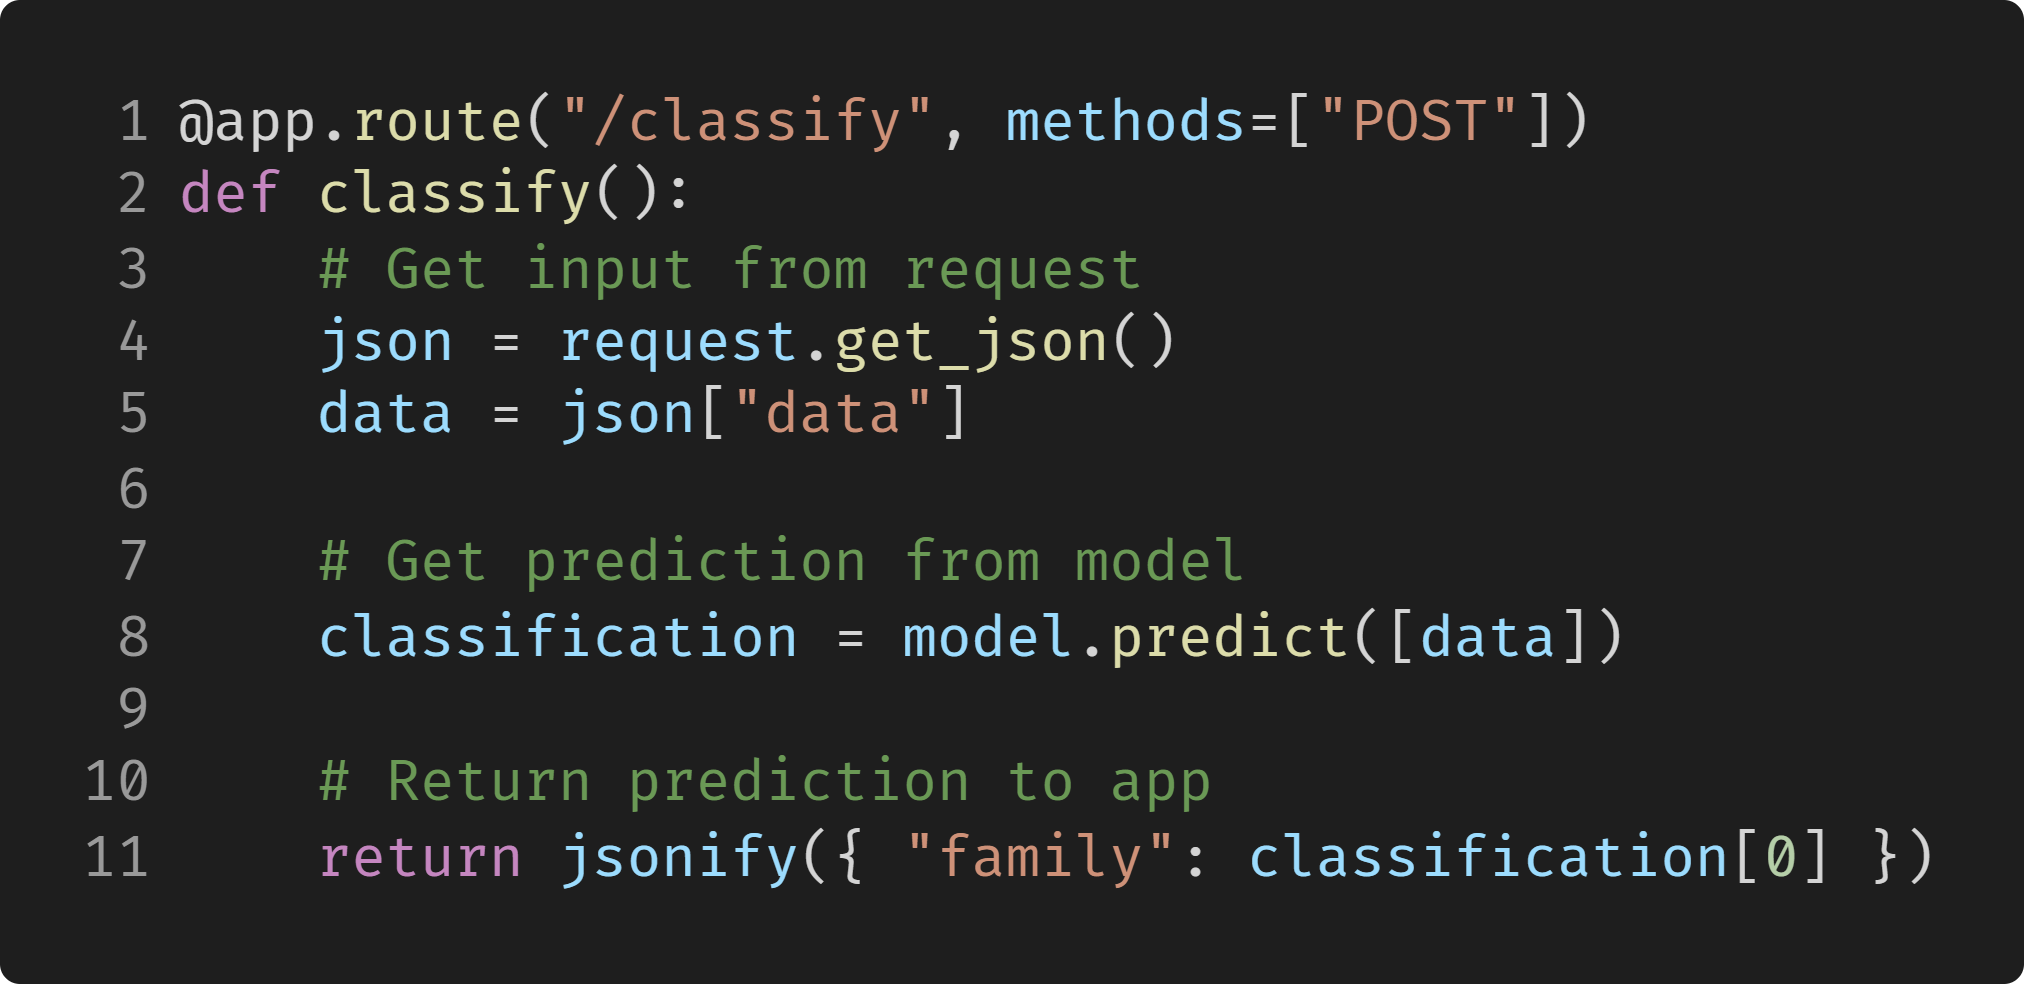
\includegraphics[width=.75\textwidth]{chapter-4/step-8-deploy-model.png}
  \caption{Model uitgerold met behulp van een \Acrshort{api}.}
  \label{fig:step-8-deploy-model}
\end{figure}

\subsection{Stap 9: Feedback loop (Model feedback)}\label{subsec:feebdack-loop}
Om het model continue te verbeteren kan feedback verzameld worden. De feedback geeft een beeld van de effectiviteit van het model in een productie omgeving. Feedback kan verdeeld worden in twee soorten: impliciet en expliciet \cite[p.~264]{introduction-to-machine-learning}.

Het verzamelen van impliciete feedback wordt gedaan zonder dat de gebruiker zich daar bewust van is. Dit wordt gedaan door bij te houden of een voorspelling geschikt is. Een voorbeeld van deze methode is het bijhouden of een gebruiker een video kijkt dat door het algoritme voorgesteld is.

In tegenstelling tot impliciet wordt bij expliciete feedback gevraagd aan de gebruiker of een voorspelling gepast is. Een voorbeeld van deze vorm in de praktijk is hoe YouTube expliciete feedback vraagt (\autoref{fig:step-9-explicit-feedback}). Naast het aangeven of de voorspelling gepast was, kan de gebruiker ook aangeven waarom de video gepast was.

\begin{figure}[hbt!]
  \centering
  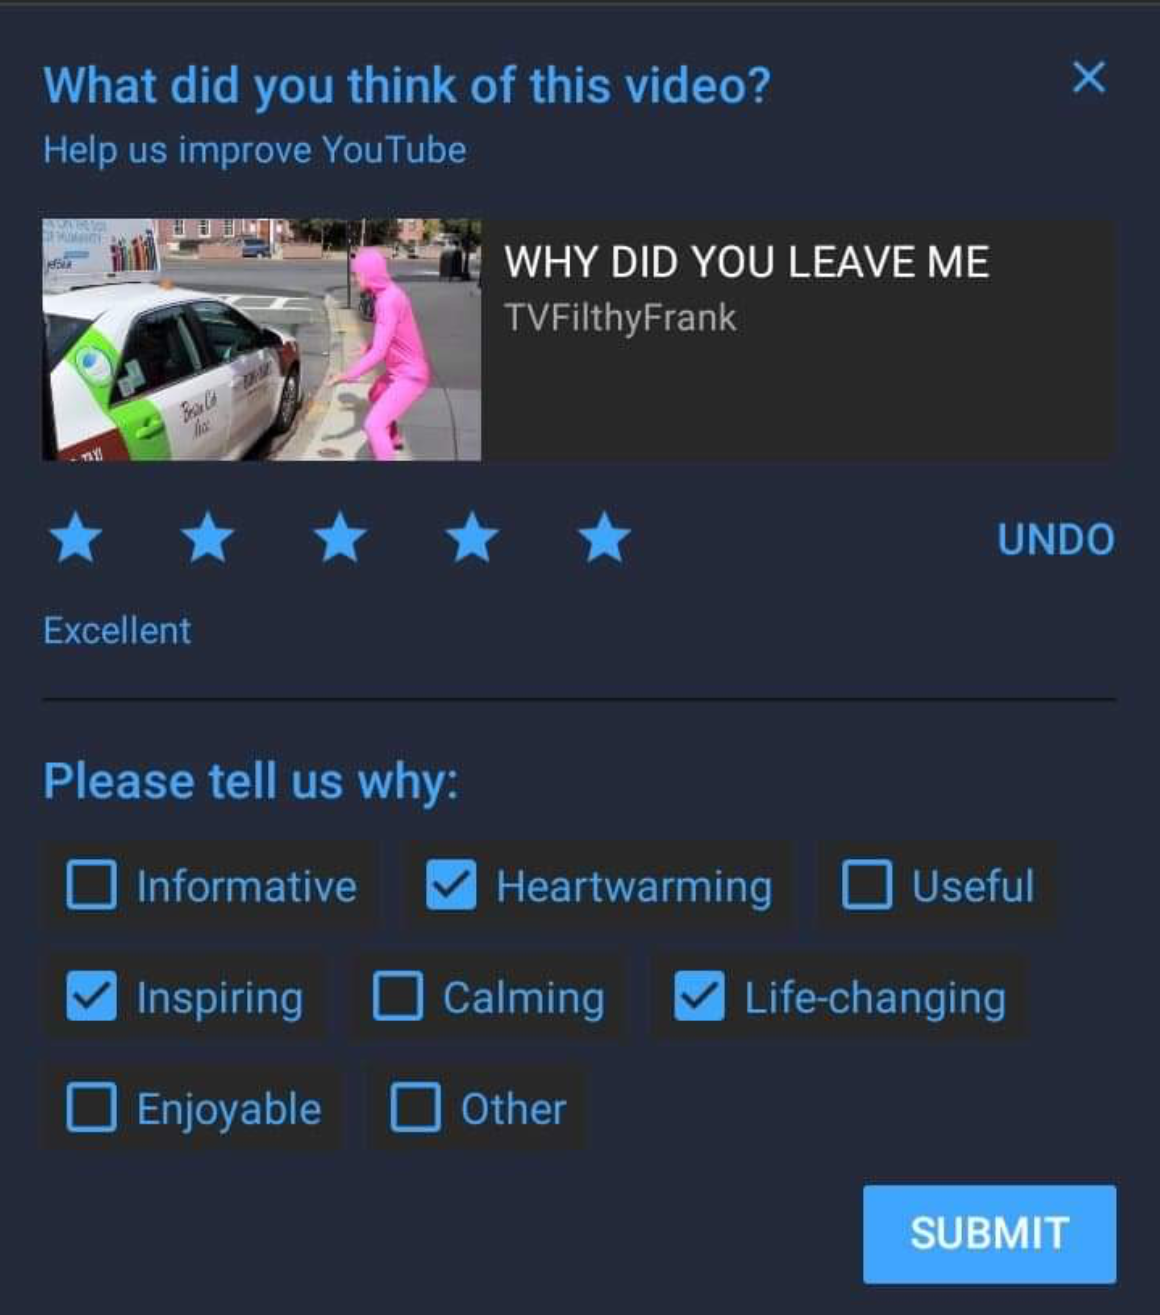
\includegraphics[width=.5\textwidth]{chapter-4/step-9-explicit-feedback.png}
  \caption{Vorm van expliciete feedback gebruikt door YouTube.}
  \label{fig:step-9-explicit-feedback}
\end{figure}

Het verzamelen van feedback is niet noodzakelijk maar helpt met het verbeteren van het model. Deze stap gaat samen met een nieuwe dataset naar de eerste stap in de lifecycle (\autoref{fig:model-lifecycle-oreilly}). Met de nieuwe dataset en de feedback kan een nieuw model getraind worden dat beter presteert dan de voorganger.

\section{Conclusie}\label{conclusie}
In dit hoofdstuk is er onderzoek gedaan naar de antwoord op de deelvraag: \textbf{D1: Waar bestaat een machine learning pipeline uit?} Het onderzoek is uitgevoerd met behulp van zowel digitale bronnen als een boek.

Een ML pipeline bestaat uit verschillende stappen die op hun beurt bestaan uit acties. De stappen zijn gericht op het waarborgen van de kwaliteit van de dataset en model, het voorbereiden van de dataset en het trainen van het model. Daarnaast kan het model uitgerold worden in een productie omgeving en kan er feedback verzameld worden over de prestatie van het model volgens gebruikers.

De acties in de stappen moeten bij het eerste gebruik van de pipeline gedefinieerd worden. De acties kan bijvoorbeeld het filteren van onbruikbare data, een model trainen of statistieken genereren zijn, Als dit vast staat, kan de pipeline hergebruikt worden om nieuwe modellen te trainen met nieuwe datasets. Op deze manier is een ML pipeline een gestructureerde en reproduceerbare proces.

\section{Advies}\label{advies}
Het in gebruik nemen van een ML pipeline werkwijze is initieel ingewikkeld maar lonend op lange termijn. Het opzetten van de pipeline en de acties definiëren kost tijd en kennis. Echter als dit eenmaal gedaan is, kan eenvoudig een verbeterd model worden getraind door een nieuwe dataset aan te leveren. Een verbeterd model is vrijwel gegarandeerd omdat stappen in de pipeline de dataset en het model analyseren en valideren.

\subsection{Machine learning pipeline verbeteringen}\label{subsec:machine-learning-pipeline-verbeteringen}
Zoals eerder aangegeven in \autoref{sec:wat-is-machine-learning} bestaat er niet één ML pipeline dat correct is. Een ML pipeline is een werkwijze waarbij de stappen anders geïnterpreteerd kan worden. Hierdoor is er geen regelmaat tussen verschillende pipelines. Dit is ook niet haalbaar aangezien stappen gemaakt kunnen worden dat specifiek is voor het algoritme of workflow van het bedrijf. De stappen in de pipeline van Hapke en Nelson (\autoref{fig:model-lifecycle-oreilly}) is een valide basis maar kan uitgebreid worden om de ervaring van developers te verbeteren. In stap 4 en 5 (\autoref{subsec:model-trainen-en-tunen}) wordt een model getraind waarbij het beste algoritme om het ML probleem op te lossen al bekend is. De verwachting is dat de keuze/onderzoek vóór het starten van de pipeline is gedaan. Tussen stap 3 en 4 kan echter een stap tussen zitten om te experimenteren met een combinatie van verschillende algoritmes en hyperparameters. In \autoref{fig:advice-ml-pipeline-lifecycle-v1} is te zien hoe zo een stap zou passen in de lifecycle. De stap is met een stippellijn aangegeven omdat de stap de eerste keer meegenomen kan worden als de pipeline wordt doorlopen. Na de eerste keer is de beste algoritme en hyperparameters al bekend en kan deze stap overgeslagen worden.

\begin{figure}[hbt!]
  \centering
  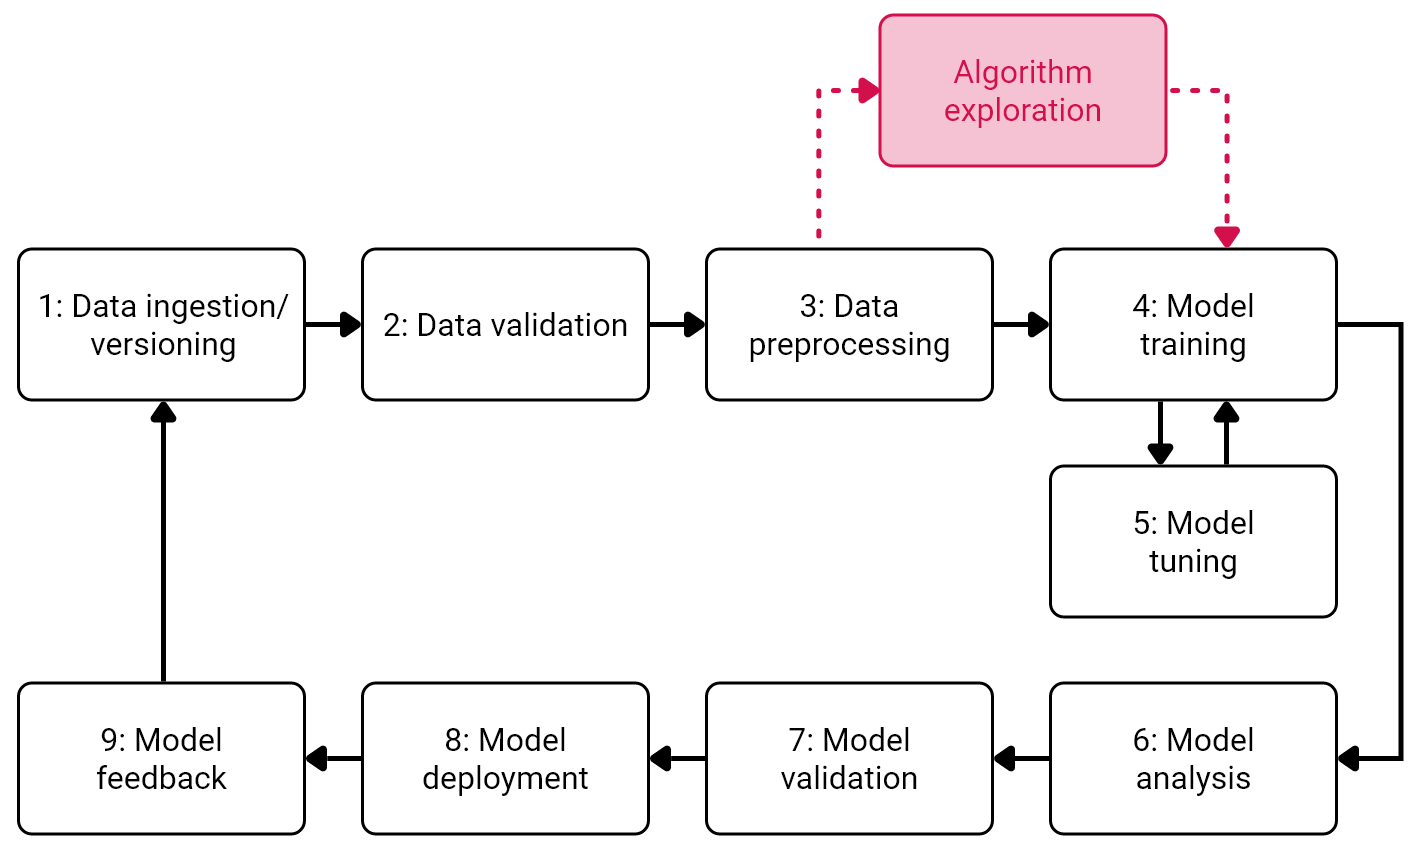
\includegraphics[width=.8\textwidth]{chapter-4/advice-ml-pipeline-lifecycle-v1.png}
  \caption{Machine learning pipeline met een algoritme exploratie tussenstap.}
  \label{fig:advice-ml-pipeline-lifecycle-v1}
\end{figure}

In de "Algorithm exploration"\space stap kunnen verschillende algoritmes dat hetzelfde doel bereiken en een variatie van hyperparameters voor elk algoritme getest worden tegen het dataset. Uit deze tests kan een prestatiescore gegenereerd worden om vervolgens te kiezen voor het algoritme dat het geschiktst lijkt. Na de keuze kan de pipeline verder gaan met de volgende stappen.

\subsection{Machine learning versimpelen}\label{subsec:machine-learning-versimpelen}
Een van de focuspunten is om te onderzoeken in hoeverre ML te vergemakkelijken is voor developers. Met de huidige pipeline is er vrij veel kennis vereist over ML om ermee te werken. Toch kan een groot deel van de stappen geautomatiseerd worden. Tussen elke stap kan een validatie plaatsvinden met een aantal randvoorwaardes waaraan voldaan moeten worden om door te gaan naar de volgende stap. In \autoref{fig:advice-ml-pipeline-lifecycle-v3} is te zien hoe tussen elke stap een validatie plaats vindt. Om bijvoorbeeld van stap 6 (Model analysis) naar stap 7 (Model validation) te gaan, moet het model even goed of zelfs beter presteren dan de voorganger. Hoe veel beter het model moet kunnen presteren is aan een developer. Mocht het zo zijn dat het model niet voldoet, kan de pipeline stopgezet worden.

\begin{figure}[hbt!]
  \centering
  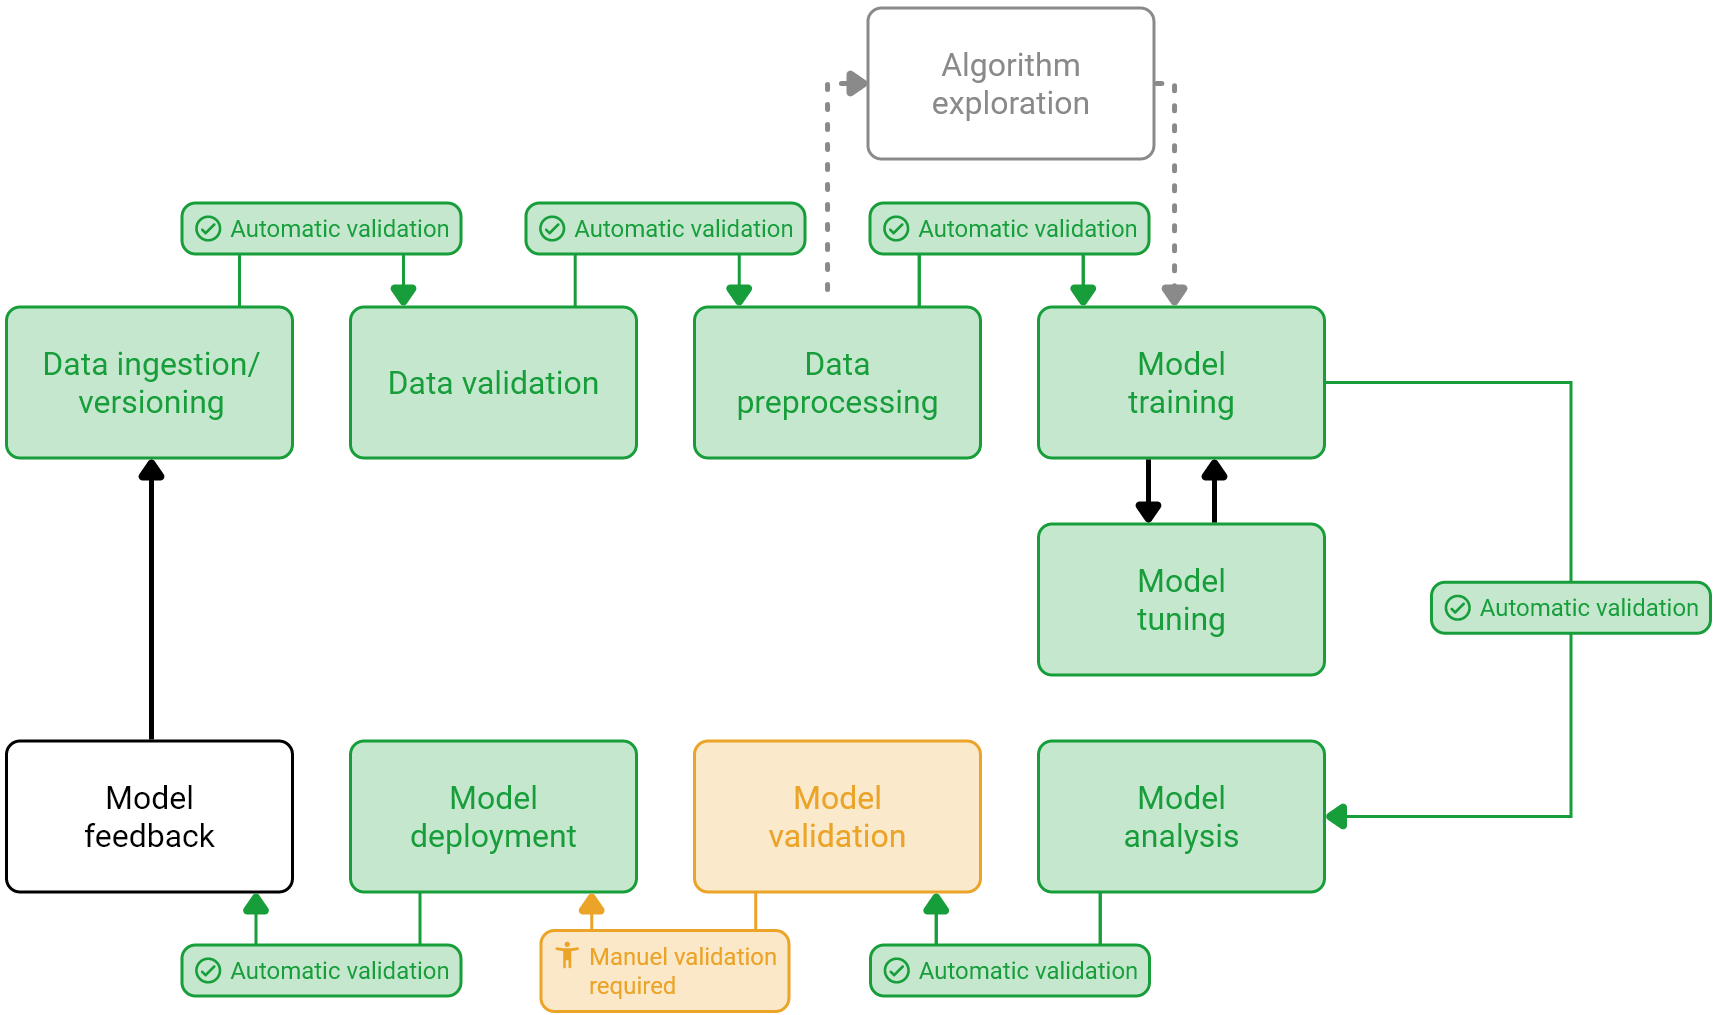
\includegraphics[width=.9\textwidth]{chapter-4/advice-ml-pipeline-lifecycle-v3.png}
  \caption{Machine learning pipeline waarbij stappen geautomatiseerd kunnen worden voor het gemak van developers.}
  \label{fig:advice-ml-pipeline-lifecycle-v3}
\end{figure}

Niet alle aspecten van de pipeline kunnen versimpelt worden. Een van de stappen dat niet kan is stap 7 (Model validation) in \autoref{fig:advice-ml-pipeline-lifecycle-v3}. Deze stap vereist input van een mens aangezien de bias van het model wordt beoordeelt. Wel kunnen rapporten over de bias gegenereerd worden zodat de workflow van developers gestroomlijnd wordt.
\styledchapter[Cloud computing platformen]{cloud-computing-platformen}
\styledchapter[Frameworks om platformen te beheren]{frameworks-beheren-platformen}
\styledchapter[Architecturale ontwerp van de oplossing]{architecturale-ontwerp}

\section{Literatuur}

\section{Design}

\section{Conclusie}
\styledchapter[Oplossing]{oplossing}

\section{Scope definiëren}

\section{Research techstack}

\section{Wireframe}

\section{Mockup}

\section{POC}

\section{Conclusie}
\styledchapter[Conclusie]{conclusie}

\cleardoublepage
\styledchapter[Aanbeveling]{aanbeveling}
\styledchapter[Discussie]{discussie}
\styledchapter[Reflectie]{reflectie}

\section{Deelvraag 1: Hoe werkt Machine Learning?}

% Bibliography
\styledunmarkedchapter[\bibname]{bibliografie}
\printbibliography[heading=none]

% Appendix input
\renewcommand{\appendixname}{Bijlagen}
\renewcommand{\appendixtocname}{Bijlagen}
\renewcommand{\appendixpagename}{Bijlagen}
\appendix
\renewcommand{\thesection}{Bijlage \arabic{section}}
\setcounter{chapter}{0}
\setcounter{section}{0}
\setcounter{subsection}{0}
\styledunmarkedchapter[Bijlagen]{bijlagen}

\section*{Scope hoofd- en deelvragen}\label{appendix:scope-subquestions-and-main-question}

\subsection*{Scope deelvraag 1}\label{appendix:scope-subquestion-1}
\begin{table}[hbt!]
  \centering
  \begin{tabular}{|p{.215\linewidth}|p{.72\linewidth}|}
  \hline
  \multicolumn{2}{|p{.97\linewidth}|}{\textbf{D1: Uit welke stappen bestaat een machine learning pipeline?}} \\ \hline
    \textbf{Scope}&
      Binnen de scope:
      \begin{itemize}
        \item In kaart brengen uit welke stappen een pipeline bestaat
        \item Acties die in een stap worden uitgevoerd
        \item Of het mogelijk is om stappen te versimpelen / abstraheren voor developers
        \item Of het mogelijk is om stappen en acties te automatiseren
      \end{itemize}
      Buiten de scope:
      \begin{itemize}
        \item Automatisering van stappen en acties
        \item Een versimpeling van machine learning
      \end{itemize}
    \\ \hline
    \textbf{Toelichting}&
      Er wordt gekeken naar welke stappen er in een pipeline zitten. De theorie wordt vervolgens toegepast in een experiment. De nadruk ligt vooral of de mogelijkheid er is om stappen en acties te automatiseren en of machine learning versimpeld kan worden, niet dat er een uitwerking is.
    \\ \hline
  \end{tabular}
  \caption{Scope deelvraag 1}
  \label{table:scope-subquestion-1}
\end{table}

\newpage

\subsection*{Scope deelvraag 2}\label{appendix:scope-subquestion-2}
\begin{table}[hbt!]
  \centering
  \begin{tabular}{|p{.215\linewidth}|p{.72\linewidth}|}
  \hline
  \multicolumn{2}{|p{.97\linewidth}|}{\textbf{D2: Hoe kan een framework verschillende cloud computing platformen beheren om een machine learning pipeline op te zetten?}} \\ \hline
    \textbf{Scope}&
      Binnen de scope:
      \begin{itemize}
        \item High-level uitleg over hoe een framework werkt
        \item Inventarisatie met de "knock-out"\space methode
        \item Criteria lijst voor frameworks
        \item Opmerkelijke features die relevant zijn voor de PoC
        \item Ervaring opdoen doormiddel van een pipeline te maken op twee cloud computing platformen
      \end{itemize}
      Buiten de scope:
      \begin{itemize}
        \item Performance en snelheid
      \end{itemize}
    \\ \hline
    \textbf{Toelichting}&
      Frameworks dat cloud computing platformen beheert worden in kaart gebracht. Met knock-out criteria wordt de lijst verkort. Met een framework wordt een pipeline opgezet.
    \\ \hline
  \end{tabular}
  \caption{Scope deelvraag 2}
  \label{table:scope-subquestion-2}
  \end{table}

\subsection*{Scope deelvraag 3}\label{appendix:scope-subquestion-3}
\begin{table}[hbt!]
  \centering
  \begin{tabular}{|p{.215\linewidth}|p{.72\linewidth}|}
  \hline
  \multicolumn{2}{|p{.97\linewidth}|}{\textbf{D3: Hoe ziet de architecturale blauwdruk van een applicatie, waarmee een platform-onafhankelijk machine learning pipeline opgezet kan worden, eruit?}} \\ \hline
    \textbf{Scope}&
      Binnen de scope:
      \begin{itemize}
        \item Technische tekeningen
      \end{itemize}
      Buiten de scope:
      -
    \\ \hline
    \textbf{Toelichting}&
      De literatuuronderzoek slaat op of de technische tekeningen gemaakt zijn volgens een standaard zoals UML. Dit komt niet terug als theorie maar de bronnen worden wel vermeld.
    \\ \hline
  \end{tabular}
  \caption{Scope deelvraag 3}
  \label{table:scope-subquestion-3}
\end{table}

\newpage

\subsection*{Scope hoofdvraag}\label{appendix:scope-main-question}
\begin{table}[hbt!]
  \centering
  \begin{tabular}{|p{.215\linewidth}|p{.72\linewidth}|}
  \hline
  \multicolumn{2}{|p{.97\linewidth}|}{\textbf{H: In welke mate kan een machine learning pipeline worden geautomatiseerd onafhankelijk van de onderliggende cloud computing platform?}} \\ \hline
    \textbf{Scope}&
      De scope wordt bepaald na de requirement analyse.
    \\ \hline
    \textbf{Toelichting}&
      Onderzoek naar documentatie van gebruikte framework(s).
    \\ \hline
  \end{tabular}
  \caption{Scope hoofdvraag}
  \label{table:scope-main-question}
\end{table}

\newpage
\section*{Criteria met toelichting voor cloud computing platformen}\label{appendix:criteria-with-elaboration-for-cloud-computing-platforms}

\begin{table}[hbt!]
  \centering
  \caption{Criteria voor cloud computing platformen}
  \begin{tabular}{|p{.2\linewidth}|p{.69\linewidth}|}
  \hline
  \textbf{Criteria} & \textbf{Toelichting} \\ \hline
    ML Pipeline \newline aanmaken
    &
    Het platform moet het aanmaken van een machine learning pipeline kunnen ondersteunen. 
    \\ \hline

    Serverbeheer
    &
    Aanmaken, wijzigen en verwijderen van een server. Een server kunnen aanmaken bij het platform is praktisch omdat een server voor meerdere doeleinde gebruikt kan worden.
    \\ \hline

    Database beheer
    &
    Aanmaken, wijzigen en verwijderen van een database. De PoC moet data ergens kunnen opslaan en vandaan halen; dit is mogelijk in een database.
    \\ \hline

    Storage \newline bucket beheer
    &
    Aanmaken, wijzigen en verwijderen van een storage bucket. In een storage bucket kan grote hoeveelheden data opgeslagen worden zoals bestanden en afbeeldingen. Dit kan handig zijn om bijvoorbeeld train en test data op te slaan.
    \\ \hline

    Uptime 99.9\%
    &
    Het platform moet een vorm van uptime kunnen garanderen waarbij het percentage zo dicht mogelijk bij 99.9 ligt. Hierdoor is de kans dat NGTI door een storing bij een platform niet productief kan zijn zo klein mogelijk.
    \\ \hline

    Regionale \newline beschikbaarheid
    &
    Waar data wordt opgeslagen en de servers draaien is vrij belangrijk. Het platform moet ten minste West-Europa ondersteunen in verband met de gegevensbescherming in de EU (GDPR). In een ideale situatie zou het platform ook specifiek Zwitserland ondersteunen aangezien de meeste klanten van NGTI vandaar komen.
    \\ \hline

    Toegankelijkheid documentatie ML pipeline
    &
    In het geval dat de PoC wordt uitgebreid tot een applicatie is het belangrijk om onderhoud uit te voeren en eventueel nieuwe functies toe te voegen. Het is daarom van belang dat het platform documentatie heeft over ML pipelines. 
    \\ \hline

    APIs
    &
    Om het platform programmatisch aan te sturen zijn APIs dat het platform beschikbaar stelt onmisbaar. Op deze manier kunnen frameworks het platform beheren en kan eventueel een op maat gemaakte oplossing gebruikt worden.
    \\ \hline

    Inhoud ML
    &
    Voor NGTI is het belangrijk dat het platform niet alleen ondersteuning heeft om modellen te trainen, maar meer mogelijkheden biedt zoals het schrijven van een eigen algoritme of out-of-the-box oplossingen.
    \\ \hline
  \end{tabular}
  \label{table:criteria-cloud-computing-platforms}
\end{table}

\newpage
\section*{Gedetailleerd overzicht cloud computing platformen}\label{appendix:detailed-overview-of-cloud-computing-platforms}

\subsection*{AWS}\label{appendix:detailed-overview-of-cloud-computing-platforms:aws}
\begin{table}[hbt!]
  \centering
  \begin{tabular}{|p{.2\linewidth}|p{.74\linewidth}|}
  \hline
  \textbf{Criteria} & \textbf{Toelichting} \\ \hline
    ML Pipeline \newline aanmaken
    &
    Met \underline{\href{https://aws.amazon.com/sagemaker/pipelines/}{Amazon SageMaker}} kunnen pipelines gemaakt worden. Daarnaast heeft Amazon specifieke services om bijvoorbeeld vooroordelen te detecteren, statistieken te meten en data te verzamelen (\underline{\href{https://aws.amazon.com/machine-learning/}{overzicht}}).
    \\ \hline

    Serverbeheer
    &
    Met \underline{\href{https://aws.amazon.com/ec2/}{Amazon EC2}} kunnen servers worden opgestart, gewijzigd of verwijderd worden. Een \underline{\href{https://aws.amazon.com/ec2/features/}{overzicht}} wat Amazon EC2 allemaal kan
    \\ \hline

    Database beheer
    &
    Amazon biedt een database service aan waarbij een database aangemaakt, gewijzigd of verwijderd kan worden. De databases zijn gesorteerd op type in dit \underline{\href{https://aws.amazon.com/products/databases/?nc2=h_ql_prod_db}{overzicht}}.
    \\ \hline

    Storage \newline bucket beheer
    &
    Wat betreft opslag biedt Amazon twee soorten aan: \underline{\href{https://aws.amazon.com/s3}{Amazon S3}} en \underline{\href{https://aws.amazon.com/ebs}{Amazon Elastic Block Store}}. Het verschil is dat S3 data opslaat als een object ten opzicht van Elastic Block Storage, dat data op de conventionele manier opslaat.
    \\ \hline

    Uptime 99.9\%
    &
    De uptime staat beschreven in de Service Level Agreement (SLA) en is voor elke service anders. Over het algemeen biedt Amazon voor elke service een uptime van 99.9\%: \underline{\href{https://aws.amazon.com/sagemaker/sla/}{Amazon SageMaker}}, \underline{\href{https://aws.amazon.com/compute/sla/}{Amazon EC2 en Elastic Block Store}}, \underline{\href{https://aws.amazon.com/rds/sla/}{Amazon Relational Databases}} en \underline{\href{https://aws.amazon.com/s3/sla/}{Amazon S3}}.
    \\ \hline

    Regionale \newline beschikbaarheid
    &
    Amazon heeft in totaal zes fysieke datacenters in Europa (\underline{\href{https://aws.amazon.com/about-aws/global-infrastructure/regions_az/}{overzicht}}). Ook is het mogelijk om een specifiek regio te kiezen zoals het \underline{\href{https://docs.aws.amazon.com/AWSEC2/latest/UserGuide/using-regions-availability-zones.html\#using-regions-availability-zones-setup}{hier}} beschreven staat. Helaas is Zwitserland geen beschikbare regio.
    \\ \hline

    Toegankelijkheid documentatie ML pipeline
    &
    Amazon heeft een uitgebreide services voor ML binnen AWS. Alle services zijn te vinden in dit \underline(\href{https://aws.amazon.com/machine-learning/}{overzicht}).
    \\ \hline

    APIs
    &
    Voor al haar services stelt Amazon een API beschikbaar. Een overzicht voor de documentatie is \underline{\href{https://docs.aws.amazon.com/index.html?nc2=h_ql_doc_do_v}{hier}} te vinden. API documentatie voor \underline{\href{https://docs.aws.amazon.com/machine-learning/}{ML}} en \underline{\href{https://docs.aws.amazon.com/sagemaker/}{SageMaker}} is ook beschikbaar.
    \\ \hline

    Inhoud ML
    &
    Amazon heeft een groot aantal ML specifieke services waar gebruik van gemaakt kan worden. Een paar voorbeelden daarvan is \underline{\href{https://aws.amazon.com/translate/}{Amazon Translate}}, \underline{\href{https://aws.amazon.com/healthlake/}{Amazon Healthlake}} en \underline{\href{https://aws.amazon.com/forecast/}{Amazon Forecast}}.
    \\ \hline
  \end{tabular}
  \caption{AWS tegenover criteria op 06-04-2021}
  \label{table:aws-against-criteria}
\end{table}

\newpage

\subsection*{Azure}\label{appendix:detailed-overview-of-cloud-computing-platforms:azure}
\begin{table}[hbt!]
  \centering
  \begin{tabular}{|p{.2\linewidth}|p{.74\linewidth}|}
  \hline
  \textbf{Criteria} & \textbf{Toelichting} \\ \hline
    ML Pipeline \newline aanmaken
    &

    \\ \hline

    Serverbeheer
    &

    \\ \hline

    Database beheer
    &

    \\ \hline

    Storage \newline bucket beheer
    &

    \\ \hline

    Uptime 99.9\%
    &

    \\ \hline

    Regionale \newline beschikbaarheid
    &

    \\ \hline

    Toegankelijkheid documentatie ML pipeline
    &

    \\ \hline

    APIs
    &

    \\ \hline

    Inhoud ML
    &

    \\ \hline
  \end{tabular}
  \caption{Azure tegenover criteria op 06-04-2021}
  \label{table:azure-against-criteria}
\end{table}

\newpage

\subsection*{Google Cloud}\label{appendix:detailed-overview-of-cloud-computing-platforms:google-cloud}
\begin{table}[hbt!]
  \centering
  \begin{tabular}{|p{.2\linewidth}|p{.74\linewidth}|}
  \hline
  \textbf{Criteria} & \textbf{Toelichting} \\ \hline
    ML Pipeline \newline aanmaken
    &

    \\ \hline

    Serverbeheer
    &

    \\ \hline

    Database beheer
    &

    \\ \hline

    Storage \newline bucket beheer
    &

    \\ \hline

    Uptime 99.9\%
    &

    \\ \hline

    Regionale \newline beschikbaarheid
    &

    \\ \hline

    Toegankelijkheid documentatie ML pipeline
    &

    \\ \hline

    APIs
    &

    \\ \hline

    Inhoud ML
    &

    \\ \hline
  \end{tabular}
  \caption{Google Cloud tegenover criteria op 06-04-2021}
  \label{table:google-cloud-against-criteria}
\end{table}

\newpage

\subsection*{DigitalOcean}\label{appendix:detailed-overview-of-cloud-computing-platforms:digitalocean}
\begin{table}[hbt!]
  \centering
  \begin{tabular}{|p{.2\linewidth}|p{.74\linewidth}|}
  \hline
  \textbf{Criteria} & \textbf{Toelichting} \\ \hline
    ML Pipeline \newline aanmaken
    &

    \\ \hline

    Serverbeheer
    &

    \\ \hline

    Database beheer
    &

    \\ \hline

    Storage \newline bucket beheer
    &

    \\ \hline

    Uptime 99.9\%
    &

    \\ \hline

    Regionale \newline beschikbaarheid
    &

    \\ \hline

    Toegankelijkheid documentatie ML pipeline
    &

    \\ \hline

    APIs
    &

    \\ \hline

    Inhoud ML
    &

    \\ \hline
  \end{tabular}
  \caption{DigitalOcean tegenover criteria op 06-04-2021}
  \label{table:digitalocean-against-criteria}
\end{table}

\newpage

\subsection*{IBM Cloud}\label{appendix:detailed-overview-of-cloud-computing-platforms:ibm-cloud}
\begin{table}[hbt!]
  \centering
  \begin{tabular}{|p{.2\linewidth}|p{.74\linewidth}|}
  \hline
  \textbf{Criteria} & \textbf{Toelichting} \\ \hline
    ML Pipeline \newline aanmaken
    &

    \\ \hline

    Serverbeheer
    &

    \\ \hline

    Database beheer
    &

    \\ \hline

    Storage \newline bucket beheer
    &

    \\ \hline

    Uptime 99.9\%
    &

    \\ \hline

    Regionale \newline beschikbaarheid
    &

    \\ \hline

    Toegankelijkheid documentatie ML pipeline
    &

    \\ \hline

    APIs
    &

    \\ \hline

    Inhoud ML
    &

    \\ \hline
  \end{tabular}
  \caption{IBM Cloud tegenover criteria op 06-04-2021}
  \label{table:ibm-cloud-against-criteria}
\end{table}

\newpage

\subsection*{Alibaba}\label{appendix:detailed-overview-of-cloud-computing-platforms:alibaba}
\begin{table}[hbt!]
  \centering
  \begin{tabular}{|p{.2\linewidth}|p{.74\linewidth}|}
  \hline
  \textbf{Criteria} & \textbf{Toelichting} \\ \hline
    ML Pipeline \newline aanmaken
    &

    \\ \hline

    Serverbeheer
    &

    \\ \hline

    Database beheer
    &

    \\ \hline

    Storage \newline bucket beheer
    &

    \\ \hline

    Uptime 99.9\%
    &

    \\ \hline

    Regionale \newline beschikbaarheid
    &

    \\ \hline

    Toegankelijkheid documentatie ML pipeline
    &

    \\ \hline

    APIs
    &

    \\ \hline

    Inhoud ML
    &

    \\ \hline
  \end{tabular}
  \caption{Alibaba tegenover criteria op 06-04-2021}
  \label{table:alibaba-against-criteria}
\end{table}

\newpage

\subsection*{Oracle Cloud Infrastructure}\label{appendix:detailed-overview-of-cloud-computing-platforms:oracle-cloud-infrastructure}
\begin{table}[hbt!]
  \centering
  \begin{tabular}{|p{.2\linewidth}|p{.74\linewidth}|}
  \hline
  \textbf{Criteria} & \textbf{Toelichting} \\ \hline
    ML Pipeline \newline aanmaken
    &

    \\ \hline

    Serverbeheer
    &

    \\ \hline

    Database beheer
    &

    \\ \hline

    Storage \newline bucket beheer
    &

    \\ \hline

    Uptime 99.9\%
    &

    \\ \hline

    Regionale \newline beschikbaarheid
    &

    \\ \hline

    Toegankelijkheid documentatie ML pipeline
    &

    \\ \hline

    APIs
    &

    \\ \hline

    Inhoud ML
    &

    \\ \hline
  \end{tabular}
  \caption{Oracle Cloud Infrastructure tegenover criteria op 06-04-2021}
  \label{table:oracle-cloud-infrastructure-against-criteria}
\end{table}

\newpage

\subsection*{Kamatera Cloud}\label{appendix:detailed-overview-of-cloud-computing-platforms:katamara-cloud}
\begin{table}[hbt!]
  \centering
  \begin{tabular}{|p{.2\linewidth}|p{.74\linewidth}|}
  \hline
  \textbf{Criteria} & \textbf{Toelichting} \\ \hline
    ML Pipeline \newline aanmaken
    &

    \\ \hline

    Serverbeheer
    &

    \\ \hline

    Database beheer
    &

    \\ \hline

    Storage \newline bucket beheer
    &

    \\ \hline

    Uptime 99.9\%
    &

    \\ \hline

    Regionale \newline beschikbaarheid
    &

    \\ \hline

    Toegankelijkheid documentatie ML pipeline
    &

    \\ \hline

    APIs
    &

    \\ \hline

    Inhoud ML
    &

    \\ \hline
  \end{tabular}
  \caption{Kamatera Cloud tegenover criteria op 06-04-2021}
  \label{table:kamatera-cloud-against-criteria}
\end{table}

\newpage

\subsection*{Cloudways}\label{appendix:detailed-overview-of-cloud-computing-platforms:cloudways}
\begin{table}[hbt!]
  \centering
  \begin{tabular}{|p{.2\linewidth}|p{.74\linewidth}|}
  \hline
  \textbf{Criteria} & \textbf{Toelichting} \\ \hline
    ML Pipeline \newline aanmaken
    &

    \\ \hline

    Serverbeheer
    &

    \\ \hline

    Database beheer
    &

    \\ \hline

    Storage \newline bucket beheer
    &

    \\ \hline

    Uptime 99.9\%
    &

    \\ \hline

    Regionale \newline beschikbaarheid
    &

    \\ \hline

    Toegankelijkheid documentatie ML pipeline
    &

    \\ \hline

    APIs
    &

    \\ \hline

    Inhoud ML
    &

    \\ \hline
  \end{tabular}
  \caption{Cloudways tegenover criteria op 06-04-2021}
  \label{table:cloudways-against-criteria}
\end{table}

\newpage

\subsection*{Vultr}\label{appendix:detailed-overview-of-cloud-computing-platforms:vultr}
\begin{table}[hbt!]
  \centering
  \begin{tabular}{|p{.2\linewidth}|p{.74\linewidth}|}
  \hline
  \textbf{Criteria} & \textbf{Toelichting} \\ \hline
    ML Pipeline \newline aanmaken
    &

    \\ \hline

    Serverbeheer
    &

    \\ \hline

    Database beheer
    &

    \\ \hline

    Storage \newline bucket beheer
    &

    \\ \hline

    Uptime 99.9\%
    &

    \\ \hline

    Regionale \newline beschikbaarheid
    &

    \\ \hline

    Toegankelijkheid documentatie ML pipeline
    &

    \\ \hline

    APIs
    &

    \\ \hline

    Inhoud ML
    &

    \\ \hline
  \end{tabular}
  \caption{Vultr tegenover criteria op 06-04-2021}
  \label{table:vultr-against-criteria}
\end{table}

\newpage

\subsection*{BigML Inc.}\label{appendix:detailed-overview-of-cloud-computing-platforms:bigml-inc}
\begin{table}[hbt!]
  \centering
  \begin{tabular}{|p{.2\linewidth}|p{.74\linewidth}|}
  \hline
  \textbf{Criteria} & \textbf{Toelichting} \\ \hline
    ML Pipeline \newline aanmaken
    &

    \\ \hline

    Serverbeheer
    &

    \\ \hline

    Database beheer
    &

    \\ \hline

    Storage \newline bucket beheer
    &

    \\ \hline

    Uptime 99.9\%
    &

    \\ \hline

    Regionale \newline beschikbaarheid
    &

    \\ \hline

    Toegankelijkheid documentatie ML pipeline
    &

    \\ \hline

    APIs
    &

    \\ \hline

    Inhoud ML
    &

    \\ \hline
  \end{tabular}
  \caption{BigML Inc. tegenover criteria op 06-04-2021}
  \label{table:bigml-inc-against-criteria}
\end{table}

\newpage

\subsection*{H2O.ai Inc.}\label{appendix:detailed-overview-of-cloud-computing-platforms:h2o.ai-inc}
\begin{table}[hbt!]
  \centering
  \begin{tabular}{|p{.2\linewidth}|p{.74\linewidth}|}
  \hline
  \textbf{Criteria} & \textbf{Toelichting} \\ \hline
    ML Pipeline \newline aanmaken
    &

    \\ \hline

    Serverbeheer
    &

    \\ \hline

    Database beheer
    &

    \\ \hline

    Storage \newline bucket beheer
    &

    \\ \hline

    Uptime 99.9\%
    &

    \\ \hline

    Regionale \newline beschikbaarheid
    &

    \\ \hline

    Toegankelijkheid documentatie ML pipeline
    &

    \\ \hline

    APIs
    &

    \\ \hline

    Inhoud ML
    &

    \\ \hline
  \end{tabular}
  \caption{H2O.ai Inc. tegenover criteria op 06-04-2021}
  \label{table:h2o.ai-inc-against-criteria}
\end{table}



\end{document}